\documentclass[11pt, spanish, a4paper]{article}

\title{Proyecto Bases de Datos}
\author{Damas Garnica Adrian \and Hernandez Barrios Samuel Rodrigo}
\date{\today}

% Configuración
\usepackage[utf8]{inputenc}
\usepackage[T1]{fontenc}
\usepackage[spanish, es-tabla]{babel}

% Paquetes básicos y de utilidades
\usepackage{abstract}
\usepackage{array}
\usepackage{amsmath}
\usepackage{booktabs}
\usepackage{caption}
\usepackage{chngcntr}
\usepackage{csquotes}
\usepackage{enumitem}
\usepackage{fancyhdr}
\usepackage{fix-cm}
\usepackage{float}
\usepackage{geometry}
\usepackage{graphicx}
\usepackage{listings}
\usepackage{parskip}
\usepackage{pgfplots}
\usepackage{subcaption}
\usepackage{tabularx}
\usepackage{tikz}
\usepackage{titlesec}
\usepackage{tocloft}
\usepackage{enumitem}
\usepackage{ragged2e}
\usepackage{url}
\usepackage{xcolor}
\usepackage{etoolbox}
\usepackage{setspace}

\usepackage{newtxsf}            % Matemáticas sans-serif a juego
\usepackage[scaled=1]{helvet}   % Helvetica/Arial
\renewcommand{\familydefault}{\sfdefault}

% Configuración de páginas y espaciado
\geometry{a4paper, margin=2.5cm}
\setstretch{1.15}          % Interlineado 1.15
\setlength{\absleftindent}{0pt}
\setlength{\absrightindent}{0pt}
\setlength{\headheight}{15.4pt}
\setlength{\parskip}{1em}
\pagestyle{plain}

% Configuración de tikz
\usetikzlibrary{trees, positioning, arrows.meta}
\pgfplotsset{compat=1.18}

% Configuración de URLs
\apptocmd{\UrlBreaks}{\do\/\do-}{}{}

% HYPERREF DEBE IR ANTES DE BIBLATEX PERO DESPUÉS DE CASI TODO
\usepackage[breaklinks=true]{hyperref}
\usepackage{xurl} % Debe ir después de hyperref

% BIBLATEX debe ir después de hyperref
% Estilo APA 7.ª edición (biblatex-apa) con citas autor-fecha
\usepackage[backend=biber, style=apa, sorting=nyt, sortcites=true, uniquename=false, backref=false]{biblatex}
\DeclareLanguageMapping{spanish}{spanish-apa}

% Configuración de hyperref
\hypersetup{
    pdftitle={Proyecto BD},
    pdfauthor={Adrian Damas Garnica, Samuel Rodrigo Hernandez Barrios},
    bookmarksopen=true
}

% Configuración de bibliografía
\addbibresource{Bibliografia.bib}
\defbibheading{bibliography}[\refname]{
    \section*{#1}
    \markboth{#1}{#1}
}

% Configuración de títulos
\titleformat{\section}
  {\normalfont\fontsize{16}{19}\bfseries\selectfont}
  {\thesection}
  {1em}
  {}
\titleformat{\subsection}
  {\normalfont\fontsize{14}{17}\bfseries\selectfont}
  {\thesubsection}
  {1em}
  {}
\titleformat{\subsubsection}
  {\normalfont\fontsize{12}{14}\bfseries\selectfont}
  {\thesubsubsection}
  {1em}
  {}

\titlespacing*{\section}{0pt}{3.5ex plus 1ex minus .2ex}{2.3ex plus .2ex}
\titlespacing*{\subsection}{0pt}{3.25ex plus 1ex minus .2ex}{1.5ex plus .2ex}
\titlespacing*{\subsubsection}{0pt}{3.25ex plus 1ex minus .2ex}{1.5ex plus .2ex}

% Configuración de encabezados
\pagestyle{fancy}
\fancyhf{}
\fancyhead[L]{\leftmark}
\fancyfoot[C]{\thepage}
\renewcommand{\headrulewidth}{0.4pt}
\renewcommand{\footrulewidth}{0pt}

% Configuración de páginas horizontales
\makeatletter
\newcommand{\intercambiarorientacion}{%
  \clearpage
  \dimen@=\dimexpr\paperwidth-\textwidth\relax
  \dimen@ii=\dimexpr\paperheight-\textheight\relax
  \global\textwidth=\dimexpr\paperheight-\dimen@\relax
  \global\textheight=\dimexpr\paperwidth-\dimen@ii\relax
  \dimen@=\paperwidth
  \global\paperwidth=\paperheight
  \global\paperheight=\dimen@
  \global\pdfpagewidth=\paperwidth
  \global\pdfpageheight=\paperheight
  \global\linewidth=\textwidth
  \global\columnwidth=\textwidth
  \global\hsize=\textwidth
  \global\headwidth=\textwidth
  \global\@colht=\textheight
  \global\@colroom=\textheight
  \global\vsize=\textheight
}
\makeatother
\newenvironment{paginahorizontal}{\intercambiarorientacion}{\intercambiarorientacion}

% Configuración de índices
\renewcommand{\cftsecleader}{\cftdotfill{\cftdotsep}}
\addto\captionsspanish{
  \renewcommand{\tablename}{Tabla}
}

% Configuración de captions
\captionsetup[figure]{name=Figura}

% Configuración de anexos
\newcounter{anexo}
\renewcommand{\theanexo}{Anexo~\arabic{anexo}}

\newenvironment{anexo}[1][]{
  \refstepcounter{anexo}
  \par\noindent\textbf{\theanexo. #1}\par
}{\par}

% Configuración de nombres especiales
\renewcommand{\abstractname}{\fontsize{12}{14}\selectfont Resumen}
\renewcommand{\lstlistlistingname}{\fontsize{12}{14}\selectfont Índice de códigos}
\renewcommand{\listtablename}{\fontsize{12}{14}\selectfont Índice de tablas}

% Configuración para código C
\lstdefinestyle{codigoC}{
    language=C,
    basicstyle=\ttfamily\footnotesize,
    keywordstyle=\color{blue}\bfseries,
    commentstyle=\color{green!50!black}\itshape,
    stringstyle=\color{red},
    numbers=left,
    numberstyle=\tiny\color{gray},
    stepnumber=1,
    numbersep=5pt,
    backgroundcolor=\color{white},
    showspaces=false,
    showstringspaces=false,
    showtabs=false,
    frame=single,
    rulecolor=\color{black},
    tabsize=4,
    captionpos=b,
    breaklines=true,
    breakatwhitespace=true,
    morekeywords={size_t, bool, true, false, pragma, omp},
    literate= % Para caracteres especiales
        {á}{{\'a}}1 {é}{{\'e}}1 {í}{{\'i}}1 {ó}{{\'o}}1 {ú}{{\'u}}1
        {Á}{{\'A}}1 {É}{{\'E}}1 {Í}{{\'I}}1 {Ó}{{\'O}}1 {Ú}{{\'U}}1
        {ñ}{{\~n}}1 {Ñ}{{\~N}}1 {¿}{{?`}}1 {¡}{{!`}}1}

% Estilo para terminal/consola
\lstdefinestyle{terminalstyle}{
    language=bash,
    basicstyle=\ttfamily\footnotesize\color{white},
    backgroundcolor=\color{black!90},
    numbers=none,
    frame=tb,
    framerule=0pt,
    framesep=3pt,
    rulecolor=\color{gray},
    xleftmargin=10pt,
    xrightmargin=10pt,
    breaklines=true,
    breakatwhitespace=true,
    showstringspaces=false,
    tabsize=2,
    % Colores para elementos específicos
    keywordstyle=\color{cyan}, % Comandos
    commentstyle=\color{green!60}, % Comentarios
    stringstyle=\color{yellow}, % Rutas y strings
    morekeywords={sudo, apt, git, python, gcc, make, cd, ls, echo}, % Comandos comunes
    morecomment=[l]{\#}, % Comentarios con #
    morestring=[b]", % Strings entre comillas
    literate= % Caracteres especiales
        {á}{{\'a}}1 {é}{{\'e}}1 {í}{{\'i}}1 {ó}{{\'o}}1 {ú}{{\'u}}1
        {Á}{{\'A}}1 {É}{{\'E}}1 {Í}{{\'I}}1 {Ó}{{\'O}}1 {Ú}{{\'U}}1
        {ñ}{{\~n}}1 {Ñ}{{\~N}}1 {¿}{{?`}}1 {¡}{{!`}}1
        {\$}{{\textcolor{green}{\$}}}1 % Prompt de terminal
        {>}{{\textcolor{green}{>}}}1   % Prompt secundario
        {*}{{\textcolor{red}{*}}}1     % Wildcards
        {~}{{\textcolor{blue}{\textasciitilde}}}1 % Directorio home
}

% Configuracion General Codigos
\renewcommand{\lstlistingname}{Código}

% Configuración para evitar underfull hboxes
\hbadness=10000
\usepackage{longtable}

% Configuracion.tex trae los datos del PDF de otro documento
\hypersetup{
    pdftitle={Proyecto Bases de Datos: Sistema de Comandas Profesional},
    pdfauthor={Damas Garnica Adrian, Hernandez Barrios Samuel Rodrigo}
}

\begin{document}

	% Portada
	\begin{titlepage}
    \centering

    % Logos
    \centering
    \begin{minipage}{0.4\textwidth}
        \centering
        \includegraphics[width=0.7\linewidth]{Imagenes/logo_ipn.png}
    \end{minipage}
    \hfill
    \begin{minipage}{0.4\textwidth}
        \centering
        \includegraphics[width=0.7\linewidth]{Imagenes/logo_escom.png}
    \end{minipage}

    % Encabezado institucional
    {\fontsize{16}{18}\selectfont \textbf{Instituto Politécnico Nacional} \par}
    \vspace{0.3cm}
    {\fontsize{14}{16}\selectfont \textbf{Escuela Superior de Cómputo} \par}
    \vspace{1.5cm}

    % Título principal
    {\Huge \textbf{Proyecto Bases de Datos} \par}
    \vspace{0.5cm}

    % Subtítulo
    {\Large\textbf{Sistema de Comandas Profesional}\par}
    \vspace*{1.5cm}

    % Información de la materia
    \begin{flushleft}
        {\large \textbf{Materia:} Bases de Datos \par}
        \vspace{0.5cm}
        {\large \textbf{Profesor:} Gabriel Hurtado Avilés \par}
        \vspace{0.5cm}
        {\large \textbf{Alumnos:} \par}
        \vspace{0.2cm}
        {\large \hspace{1em} Damas Garnica Adrian \par}
        {\large \hspace{1em} Hernandez Barrios Samuel Rodrigo \par}
        \vspace{0.5cm}
        {\large \textbf{Grupo:} 3CV4 \par}
        \vspace{0.5cm}
        {\large \textbf{Carrera:} Ingeniería en Sistemas Computacionales \par}
    \end{flushleft}

    \vfill
\end{titlepage}


	% Resumen
	\newpage
\begin{abstract}

    En este documento se recopila, de manera formal, el desarrollo de la base de datos del Sistema de Comandas Profesional realizado a lo largo de las prácticas de la materia de Bases de Datos, desde el análisis del caso de estudio y el diseño de sus modelos hasta su implementación, población y comprobación en PostgreSQL.

\end{abstract}

% El mismo resumen en inglés; el grupo limita el cambio de título a este bloque
{
\renewcommand{\abstractname}{Abstract}
\begin{abstract}

    This document formally compiles the development of the Sistema de Comandas Profesional database, carried out throughout the practices of the Databases course, from the analysis of the case study and the design of its models to its implementation, population, and verification in PostgreSQL.

\end{abstract}
}
\thispagestyle{empty}


	% Índice
	\clearpage\newpage
\pagenumbering{roman}
\tableofcontents    % Indice
\listoffigures      % Lista de figuras
\listoftables       % Lista de tablas
\lstlistoflistings  % Lista de códigos

\thispagestyle{empty}
\clearpage
\pagenumbering{arabic}
\setcounter{page}{1}


	% Introducción
	\newpage

\section{Introducción}
\label{sec:introduccion}

En esta sección se presenta el problema que da origen al proyecto, las razones que justifican el diseño de una base de datos para atenderlo, los objetivos que guiaron su desarrollo, los trabajos relacionados que se revisaron y el alcance del documento.

\subsection{Planteamiento del problema}

Los salones de eventos que ofrecen servicio de banquetes gestionan la toma y el seguimiento de las comandas, es decir, los pedidos de alimentos y bebidas que realiza cada mesa durante un evento, con comandas de papel, hojas de cálculo o aplicaciones genéricas que no fueron diseñadas para este giro. Con esta forma de operar, la información de los pedidos se duplica o se pierde entre el área de meseros, la cocina y la caja; no queda un registro histórico confiable de lo que se sirvió en cada evento ni de su costo; el inventario de insumos se controla de manera aproximada, lo que provoca faltantes o compras innecesarias; y la cuenta final de cada evento se elabora conciliando a mano varias comandas, lo que la vuelve lenta y propensa a errores.

El salón que se tomó como caso de estudio atiende alrededor de quince eventos al mes, con unas veinte mesas por evento y dos o tres cuentas por mesa. Para atenderlo, el equipo contaba con un sistema de comandas desarrollado en un semestre anterior en la materia de Sistemas Operativos: una interfaz de terminal escrita en C que guardaba la información en archivos de texto. Ese sistema carecía de relaciones bien definidas, de normalización y de reglas de integridad, de modo que cualquier cambio en el negocio obligaba a modificar el programa y nada impedía que los archivos quedaran en un estado inconsistente.

Por lo anterior, el problema que se atiende no consiste solamente en digitalizar la toma de comandas, sino en diseñar e implementar, con una metodología formal, la base de datos que sustente una versión profesional de ese sistema, capaz de representar eventos, mesas, cuentas, comandas, productos, ingredientes, personal y pagos sin perder la consistencia de la información.

\subsection{Justificación}

El sistema de comandas constituye el núcleo operativo de un salón de eventos: de él dependen la asignación de mesas, el seguimiento de los pedidos, la disponibilidad de insumos y el cobro al cliente. Un modelo de datos mal estructurado produce inconsistencias que el personal descubre hasta el cierre del evento, cuando ya no es posible corregirlas, y limita la capacidad del sistema para adaptarse a nuevos requerimientos, como los paquetes contratados, las variantes de los productos o los reportes administrativos.

Desde el punto de vista académico, el proyecto permite aplicar de forma integral los contenidos de la materia sobre un caso real y conocido por el equipo: el modelado entidad-relación y su versión extendida, la transformación al modelo relacional, la definición de datos con restricciones de dominio y de integridad referencial, el control de acceso y la manipulación de datos mediante transacciones. Contar con el sistema anterior como punto de comparación facilita identificar los errores de diseño que se cometieron y comprobar que el nuevo modelo los resuelve.

Desde el punto de vista práctico, una base de datos que hace cumplir por sí misma las reglas del negocio reduce los errores en la toma de comandas, permite conocer con precisión el consumo y las existencias de insumos y entrega cuentas correctas sin conciliación manual. Además, al concentrar las reglas en el gestor y no en el programa, cualquier aplicación que se conecte a la base, ya sea de escritorio, móvil o web, queda sujeta a las mismas validaciones.

\subsection{Objetivo general}

Diseñar, implementar y comprobar una base de datos relacional para el sistema de comandas de un salón de eventos, que gestione de manera íntegra y consistente la información de eventos, mesas, cuentas, comandas, productos, ingredientes, personal y pagos, y que sirva de sustento a la versión profesional del sistema desarrollado previamente.

\subsection{Objetivos específicos}

\begin{enumerate}[label=\arabic*.]
    \item Identificar los requerimientos de información del salón de eventos mediante una entrevista con el cliente y fundamentar los conceptos de bases de datos que guían el diseño.
    \item Construir el modelo entidad-relación del sistema y extenderlo con los conceptos del modelo entidad-relación extendido que el caso requiere.
    \item Transformar el modelo extendido en un esquema relacional mediante las reglas de transformación y ejecutarlo en PostgreSQL dentro de un contenedor de Docker.
    \item Declarar los tipos de dato, dominios, restricciones y permisos que protejan las reglas del negocio desde el propio gestor.
    \item Poblar la base de datos a partir de una fuente documentada, mediante un script de carga repetible y eficiente.
    \item Comprobar la integridad referencial y el comportamiento de las operaciones de manipulación de datos mediante pruebas y transacciones.
\end{enumerate}

\clearpage

\subsection{Estado del arte}

Para ubicar el proyecto respecto de trabajos recientes se revisaron tres estudios relacionados con los modelos de datos, la elección de un sistema gestor y la seguridad de la información. La Tabla~\ref{tab:estado-del-arte} resume cada uno y su relación con el proyecto.

\begin{table}[H]
    \centering
    \footnotesize
    \begin{tabularx}{\textwidth}
        {
            >{\RaggedRight\arraybackslash}p{2.4cm}
            >{\RaggedRight\arraybackslash}X
            >{\RaggedRight\arraybackslash}X
            >{\RaggedRight\arraybackslash}X
        }

        \toprule

        \textbf{Referencia} & \textbf{Problema y metodología} & \textbf{Resultados principales} & \textbf{Relación con el proyecto} \\

        \midrule

        \textcite{aguilar2023} &
        Revisión sistemática de la literatura sobre el modelado y la gestión de bases de datos NoSQL, sus tipos de datos y sus herramientas. &
        Identifica cuatro modelos NoSQL: clave-valor, documentos, columnas y grafos; el orientado a documentos es el más flexible y el más usado. &
        Permite contrastar los modelos NoSQL con el modelo relacional que exigen las cuentas, los pagos y las comandas. \\

        \midrule

        \textcite{taipalus2024} &
        Revisión de 117 estudios que comparan el desempeño de 44 sistemas gestores, junto con su rigor metodológico y su reproducibilidad. &
        Hay pocas comparaciones rigurosas y reproducibles; en general, los gestores NoSQL superan a los NewSQL en lectura y escritura. &
        Sustenta que la elección del gestor considere la integridad y las transacciones, y no solo el desempeño. \\

        \midrule

        \textcite{machuca2022} &
        Revisión de catorce artículos publicados entre 2016 y 2021 sobre las metodologías de seguridad en bases de datos. &
        El control de acceso es la estrategia más utilizada, seguida del cifrado y de la protección de bases de datos en la nube. &
        Respalda la definición de roles y permisos distintos para la aplicación, la consulta y la administración. \\

        \bottomrule

    \end{tabularx}
    \captionsetup{labelfont=bf, textfont=it, labelsep=newline, justification=raggedright, singlelinecheck=false}
    \caption{Trabajos relacionados con el proyecto}
    \label{tab:estado-del-arte}
\end{table}

Los tres trabajos son revisiones sistemáticas y coinciden en que ninguna tecnología de bases de datos es superior en términos absolutos: la elección depende de las necesidades del sistema. \textcite{taipalus2024} reporta que los gestores NoSQL superan a otras familias en velocidad de lectura y escritura; sin embargo, en un sistema de comandas una cuenta que no cuadra o un pago registrado dos veces afectan directamente la operación del salón, por lo que la integridad y la consistencia pesan más que la velocidad. Por esa razón se eligió PostgreSQL, un gestor relacional con soporte completo de transacciones y restricciones de integridad. De igual forma, lo reportado por \textcite{machuca2022} sobre el control de acceso se tradujo en roles con el mínimo privilegio, de modo que cada usuario de la base pueda realizar únicamente las operaciones que le corresponden.

\subsection{Alcance}

El documento abarca la base de datos del sistema de comandas en todas sus etapas: el análisis del caso de estudio, el diseño conceptual con los modelos entidad-relación y entidad-relación extendido, el diseño lógico con el modelo relacional, la implementación física en PostgreSQL, la población con datos y las pruebas de integridad y de manipulación de datos. Cada etapa corresponde a una o varias de las prácticas de la materia, y su documentación detallada, junto con los scripts y las evidencias, se encuentra en el repositorio del equipo.

Quedan fuera de este documento la aplicación que utiliza la base de datos, cuyo cliente y servidor se desarrollan por separado, y el proyecto asignado por la materia, que se documenta de forma independiente.

\subsection{Organización del documento}

Después de esta introducción, el marco teórico reúne los conceptos que sustentan el diseño y la sección de metodología describe la forma de trabajo y el entorno en que se desarrolló el proyecto. Enseguida se presentan el caso de estudio con sus requerimientos, el diseño conceptual y el diseño lógico de la base de datos. Las secciones siguientes describen su implementación en PostgreSQL, la población con datos y las pruebas de integridad referencial y de manipulación de datos. Por último, se presentan los resultados y las conclusiones del proyecto.


	% Marco teórico
	\newpage

\section{Marco teórico}
\label{sec:marco-teorico}

En esta sección se reúnen los conceptos que sustentan el diseño y la implementación de la base de datos: la noción de base de datos y de sistema gestor, las etapas de su ciclo de vida, los modelos con los que se representó el caso de estudio y los mecanismos del lenguaje SQL con los que el gestor hace cumplir las reglas del negocio.

\subsection{Dato, información y base de datos}

Un dato es un hecho que puede ser registrado y que tiene un significado implícito \parencite[p.~4]{elmasri_navathe}; por sí solo no tiene un significado más allá de su propia existencia \parencite[p.~1]{bellinger_dikw}. La información surge cuando los datos se relacionan entre sí y adquieren significado a través de esa conexión \parencite[p.~1]{bellinger_dikw}. Por ejemplo, el número de una mesa no dice nada aislado, pero ligado a un evento, a un mesero y a una cuenta permite saber quién atendió a qué grupo de invitados y cuánto consumió.

Una base de datos es, en consecuencia, una colección de datos relacionados de manera lógica y coherente, que representa algún aspecto del mundo real y que se diseña y se puebla con un propósito específico \parencite[p.~5]{elmasri_navathe}. Para \textcite{date_intro_bd}, es un sistema computarizado cuyo objetivo es llevar el registro de la información y permitir que los usuarios la consulten y la actualicen (p.~2).

\subsection{Sistema gestor de bases de datos}

Un sistema gestor de bases de datos (SGBD) es el conjunto de programas que facilita los procesos de definir, construir, manipular y compartir bases de datos entre diversos usuarios y aplicaciones \parencite[p.~6]{elmasri_navathe}. Su función es mediar entre los archivos físicos y quienes usan la información, de manera que las aplicaciones no dependan de la forma en que los datos se almacenan. Frente a los sistemas de archivos tradicionales, en los que cada programa define y mantiene sus propios archivos, un SGBD concentra la definición de los datos en un catálogo y ofrece las características que se resumen en la Tabla~\ref{tab:caracteristicas-sgbd}.

\begin{table}[H]
    \centering
    \small
    \begin{tabularx}{\textwidth}
        {
            >{\RaggedRight\arraybackslash}p{3.4cm}
            >{\RaggedRight\arraybackslash}X
        }
        \toprule
        \textbf{Característica} & \textbf{Descripción} \\
        \midrule
        Integración & Los datos se concentran en un solo repositorio en lugar de archivos independientes e inconexos. \\
        Persistencia & Los datos sobreviven a los programas que los crearon y solo cambian por una petición al gestor. \\
        Redundancia controlada & La duplicación se evita mediante la normalización y, cuando existe a propósito, el gestor mantiene las copias sincronizadas. \\
        Integridad & Los datos cumplen las restricciones declaradas en el catálogo, que el gestor valida en cada actualización. \\
        Independencia de datos & El esquema físico o lógico puede cambiar sin modificar los programas que acceden a los datos. \\
        Seguridad & Solo los usuarios autorizados pueden leer o modificar cada objeto, según los privilegios que se les otorgan. \\
        Concurrencia & Varios usuarios operan al mismo tiempo sin producir lecturas sucias ni actualizaciones perdidas. \\
        Recuperación & Tras una falla, la base regresa a un estado consistente que conserva las transacciones confirmadas. \\
        \bottomrule
    \end{tabularx}
    \captionsetup{labelfont=bf, textfont=it, labelsep=newline, justification=raggedright, singlelinecheck=false}
    \caption{Características de un sistema gestor de bases de datos}
    \label{tab:caracteristicas-sgbd}
\end{table}

Estas características se ejercen mediante cuatro sublenguajes que, en los gestores basados en SQL, conviven en una misma interfaz \parencites[pp.~38--41]{elmasri_navathe}[pp.~42--44]{silberschatz_dbconcepts}: el lenguaje de definición de datos (DDL), con el que se crean tablas, dominios y restricciones; el lenguaje de manipulación de datos (DML), con el que se insertan, modifican, borran y consultan los datos; el lenguaje de control de datos (DCL), que administra los privilegios de los usuarios; y el lenguaje de control de transacciones (TCL), que delimita las unidades de trabajo que se confirman o se descartan por completo.

Para separar las aplicaciones de los detalles de almacenamiento, los gestores siguen la arquitectura de tres niveles propuesta por el comité ANSI/SPARC \parencite[pp.~36--37]{elmasri_navathe}: el nivel interno describe cómo se almacenan los datos, el nivel conceptual describe la estructura lógica de toda la base y el nivel externo ofrece vistas con la porción de datos que interesa a cada grupo de usuarios. Gracias a esta separación, un cambio en un nivel no obliga a modificar el nivel superior ni los programas de aplicación \parencite[pp.~37--38]{elmasri_navathe}.

\subsection{Ciclo de vida de una base de datos}

Una base de datos real tiene un ciclo de vida de muchos años, durante el cual debe evolucionar conforme cambian los requerimientos \parencite[p.~8]{elmasri_navathe}. Su desarrollo se divide en etapas que van de la idea del negocio a la operación, y cada una produce un entregable que sirve de entrada a la siguiente. Este proyecto siguió esas etapas, que se describen a continuación junto con la práctica en que se trabajó cada una.

\begin{enumerate}[label=\arabic*.]
    \item \textbf{Recolección y análisis de requerimientos.} Se documenta qué información necesita la organización y qué operaciones realiza sobre ella \parencite[p.~8]{elmasri_navathe}. En el proyecto corresponde a la entrevista con el cliente de la Práctica~1.
    \item \textbf{Diseño conceptual.} Los requerimientos se expresan en un modelo semántico independiente del gestor, como el modelo entidad-relación \parencite[pp.~9--10]{chen_er_model}. Se realizó en las prácticas~1 y~2.
    \item \textbf{Diseño lógico.} El esquema conceptual se traduce al modelo del gestor elegido, por lo general el relacional, mediante reglas de transformación \parencite[p.~289]{elmasri_navathe}. Corresponde a la Práctica~3.
    \item \textbf{Diseño físico e implementación.} El esquema lógico se escribe en sentencias DDL, se ejecuta en el gestor y la base se puebla con los datos iniciales \parencites[p.~41]{date_intro_bd}[p.~31]{elmasri_navathe}. Se realizó en las prácticas~3 y~4.
    \item \textbf{Pruebas y operación.} Se comprueba que la base proteja sus reglas y se pone en uso mediante las aplicaciones \parencite[pp.~43--45]{elmasri_navathe}. Las pruebas corresponden a las prácticas~4 y~5.
\end{enumerate}

\subsection{Modelo entidad-relación y su extensión}

El modelo entidad-relación, propuesto por \textcite{chen_er_model}, representa el mundo real mediante entidades, que son los objetos de interés; atributos, que son sus propiedades; y relaciones, que son las asociaciones entre entidades. Un atributo puede ser simple o compuesto, monovaluado o multivaluado, y almacenado o derivado, cuando su valor se calcula a partir de otros datos \parencite{elmasri_navathe}. Cada relación tiene un grado, que es el número de entidades que participan en ella, y restricciones estructurales que se expresan con la notación $(\mathit{min}, \mathit{max})$: el mínimo indica si la participación de una entidad es obligatoria y el máximo, con cuántas instancias de la otra entidad puede asociarse \parencite{elmasri_navathe}.

Una entidad débil es aquella que no tiene una clave propia suficiente para identificarse y depende de una entidad propietaria a través de una relación identificadora; su clave se forma con la clave de la propietaria y una clave parcial \parencite{elmasri_navathe}. Por ejemplo, la mesa número tres solo se distingue si se sabe a qué evento pertenece.

El modelo entidad-relación extendido (EER) añade los conceptos de especialización y generalización, con los que una entidad general, o superclase, se divide en subclases que heredan sus atributos y agregan los propios \parencite{elmasri_navathe}. Una especialización está sujeta a dos restricciones: de disyunción, que indica si una instancia puede pertenecer a una sola subclase (disjunta) o a varias (solapada), y de completitud, que indica si toda instancia de la superclase debe pertenecer a alguna subclase (total) o no (parcial). El modelo extendido también contempla relaciones de grado superior, como las ternarias, que se justifican cuando ningún par de las entidades participantes determina a la tercera.

\subsection{Modelo relacional}

El modelo relacional representa la base de datos como una colección de relaciones, o tablas, en las que cada fila es una tupla y cada columna es un atributo cuyo valor pertenece a un dominio, es decir, a un conjunto de valores atómicos permitidos \parencite{elmasri_navathe}. Una clave candidata es un conjunto mínimo de atributos que identifica de forma única a cada tupla; la clave primaria es la candidata que se elige para ese fin, y una clave foránea es un conjunto de atributos que hace referencia a la clave primaria de otra relación.

Sobre estas estructuras se definen las restricciones de integridad del modelo \parencite{elmasri_navathe}: la restricción de dominio exige que cada valor pertenezca al dominio de su atributo; la de clave, que no existan dos tuplas con la misma clave; la de integridad de entidad, que la clave primaria nunca sea nula; y la de integridad referencial, que toda clave foránea haga referencia a una tupla que exista.

El paso del modelo extendido al relacional se realiza con un conjunto de reglas de transformación \parencite[p.~289]{elmasri_navathe}. Las reglas que se aplicaron en el proyecto convierten cada entidad fuerte en una tabla; descomponen los atributos compuestos en sus componentes; llevan cada atributo multivaluado a una tabla propia; transforman las relaciones uno a muchos en una clave foránea del lado de muchos, las de muchos a muchos en una tabla intermedia y las de uno a uno en una clave foránea única; convierten las relaciones de grado superior en una tabla cuya clave combina las claves de las entidades participantes; forman la clave de cada entidad débil con la de su propietaria; y representan las jerarquías con una de varias estrategias, como una tabla por superclase y una por subclase.

\subsection{Implementación en un gestor relacional}

Los conceptos anteriores se hacen cumplir en el gestor mediante las sentencias de SQL. En esta sección se describen los mecanismos de PostgreSQL que se utilizaron en el proyecto.

\subsubsection{Restricciones de dominio}

Al definir una tabla, cada columna recibe un tipo de dato y, opcionalmente, restricciones que acotan sus valores \parencite{postgres_constraints}: \texttt{NOT NULL} impide que la columna quede vacía; \texttt{DEFAULT} asigna un valor inicial cuando no se especifica uno; \texttt{UNIQUE} impide que dos filas repitan el mismo valor o combinación de valores; y \texttt{CHECK} exige que cada fila cumpla una condición, ya sea un rango, una lista de valores permitidos, un formato o una comparación entre columnas. Cuando un mismo tipo y una misma precisión se repiten en varias tablas, la sentencia \texttt{CREATE DOMAIN} permite definirlos una sola vez con un nombre propio y reutilizarlos \parencite{postgres_createdomain}.

\subsubsection{Integridad referencial}

Una clave foránea se declara con \texttt{FOREIGN KEY} y hace que el gestor rechace cualquier fila que apunte a un renglón inexistente \parencite{postgres_constraints}. La declaración incluye además una acción referencial, que determina qué ocurre con las filas hijas cuando se borra o se actualiza la fila padre: \texttt{RESTRICT} impide la operación mientras existan hijas; \texttt{CASCADE} la propaga a las hijas; \texttt{SET NULL} deja la referencia en nulo; y \texttt{SET DEFAULT} la reemplaza por un valor por omisión. La elección depende de la regla del negocio: \texttt{CASCADE} corresponde cuando la hija no tiene sentido sin su padre, como una entidad débil, y \texttt{RESTRICT} cuando el padre no debe desaparecer mientras algo dependa de él.

\subsubsection{Disparadores y vistas}

Algunas reglas del negocio relacionan varias filas o varias tablas y no pueden expresarse con una restricción de columna. Para ellas se emplean disparadores, que son funciones que el gestor ejecuta automáticamente antes o después de una inserción, actualización o borrado, y que pueden rechazar la operación o modificar los datos \parencite{postgres_triggers}. Por su parte, una vista es una consulta almacenada con un nombre, que se consulta como si fuera una tabla \parencite{postgres_createview}; se utiliza para calcular atributos derivados sin guardarlos, de modo que su valor nunca queda desactualizado, y para ofrecer a cada grupo de usuarios solo la porción de datos que necesita.

\subsubsection{Transacciones}

Una transacción es una unidad de trabajo que agrupa varias operaciones y que debe ejecutarse completa o no ejecutarse \parencite{postgres_transactions}. Las transacciones cumplen las propiedades conocidas como ACID: atomicidad, porque sus operaciones se aplican todas o ninguna; consistencia, porque llevan la base de un estado válido a otro; aislamiento, porque su ejecución no se ve afectada por otras transacciones concurrentes; y durabilidad, porque sus cambios confirmados persisten aun ante fallas \parencite{elmasri_navathe}. En SQL, una transacción inicia con \texttt{BEGIN}, se confirma con \texttt{COMMIT} y se descarta con \texttt{ROLLBACK}. Dentro de ella, \texttt{SAVEPOINT} marca un punto de recuperación al que es posible regresar con \texttt{ROLLBACK TO} sin descartar el trabajo anterior \parencite{postgres_savepoint}.

\subsubsection{Control de acceso}

El acceso a la base se administra mediante roles, que pueden representar a un usuario o a un grupo de usuarios \parencite{postgres_roles}. Con \texttt{GRANT} se otorgan privilegios sobre cada objeto, como leer, insertar, modificar o borrar en una tabla, y con \texttt{REVOKE} se retiran \parencite{postgres_privileges}. El principio de mínimo privilegio consiste en conceder a cada rol únicamente los permisos que su función requiere, de modo que un error en una aplicación o un acceso indebido no pueda afectar más datos de los necesarios.

\subsubsection{Carga masiva de datos}

Para poblar una base con volúmenes grandes de datos, insertar cada fila con una sentencia \texttt{INSERT} resulta lento, porque cada sentencia se procesa por separado. La sentencia \texttt{COPY} de PostgreSQL, y su variante \texttt{\textbackslash copy} del cliente \texttt{psql}, transfiere el contenido completo de un archivo a una tabla en una sola operación \parencite{postgres_copy}, por lo que es el mecanismo recomendado para la carga inicial de una base de datos.


	% Metodología y entorno
	\newpage

\section{Metodología y entorno de trabajo}
\label{sec:metodologia}

En esta sección se describe la forma en que se organizó el desarrollo del proyecto, las herramientas con las que el equipo coordinó su trabajo y el entorno en que se ejecutó el gestor de bases de datos.

\subsection{Desarrollo por etapas}

El proyecto se desarrolló siguiendo las etapas del ciclo de vida de una base de datos descritas en el marco teórico. Cada práctica de la materia correspondió a una o varias de esas etapas, y su resultado fue la entrada de la práctica siguiente, como se resume en la Tabla~\ref{tab:etapas}.

\begin{table}[H]
    \centering
    \small
    \begin{tabularx}{\textwidth}
        {
            >{\RaggedRight\arraybackslash}p{1.7cm}
            >{\RaggedRight\arraybackslash}p{3.6cm}
            >{\RaggedRight\arraybackslash}X
        }
        \toprule
        \textbf{Práctica} & \textbf{Etapa} & \textbf{Productos} \\
        \midrule
        1 & Requerimientos y diseño conceptual & Marco teórico, entrevista con el cliente, requerimientos, diagrama entidad-relación y entorno de trabajo con Git y Docker. \\
        2 & Diseño conceptual & Modelo entidad-relación extendido en notación de Peter Chen y análisis de los artículos del proyecto asignado. \\
        3 & Diseño lógico e implementación & Inventario del modelo extendido, reglas de transformación, esquema relacional ejecutado en PostgreSQL, diccionario de datos y pruebas de las restricciones. \\
        4 & Implementación y población & Tipos de dato y dominios, restricciones de columna, fuente de datos, script de carga, pruebas de dominio, usuarios y permisos. \\
        5 & Pruebas de integridad & Claves foráneas y acciones referenciales, pruebas de integridad, edición de valores, transacciones y experimentos individuales. \\
        \bottomrule
    \end{tabularx}
    \captionsetup{labelfont=bf, textfont=it, labelsep=newline, justification=raggedright, singlelinecheck=false}
    \caption{Etapas del ciclo de vida trabajadas en cada práctica}
    \label{tab:etapas}
\end{table}

El desarrollo no fue estrictamente lineal. Cada etapa permitió detectar omisiones de la anterior y corregirlas antes de continuar: al construir el modelo extendido se reconsideraron los requerimientos de la entrevista; al transformar el modelo al relacional se levantó primero un inventario de entidades, relaciones y atributos especiales; y al implementar las restricciones de dominio se encontraron reglas que el esquema todavía no protegía. A partir de la Práctica~4, todo cambio al esquema ya ejecutado se registró como una migración numerada con sentencias \texttt{ALTER TABLE}, en lugar de editar el script original, de modo que la historia del esquema quedara documentada y pudiera reproducirse en cualquier base.

\subsection{Control de versiones}

El código, la documentación y las evidencias del proyecto se administran con Git en un repositorio compartido en GitHub. Git registra cada cambio como una confirmación con su autor y su fecha, lo que permite reconstruir la historia del proyecto y recuperar cualquier versión anterior \parencite{chacon_progit}; GitHub agrega un repositorio remoto común y la revisión de cambios mediante \textit{pull requests} \parencite{github_repositories}.

El equipo adoptó un flujo de trabajo basado en ramas \parencite{atlassian_feature_branch}, representado en la Figura~\ref{fig:flujo-ramas}. La rama \texttt{main} contiene únicamente el trabajo revisado y entregado. Al iniciar una práctica se crea a partir de ella una rama de práctica, y cada sección de la práctica se desarrolla en una rama propia que sale de la rama de práctica. Al terminar una sección, sus cambios se integran a la rama de práctica mediante un \textit{pull request}, y al cerrar la práctica, la rama de práctica se integra a \texttt{main} con un \textit{pull request} revisado por otro integrante del equipo.

\begin{figure}[H]
    \centering
    \begin{tikzpicture}[
        rama/.style={draw, rounded corners, minimum width=3.6cm, minimum height=0.8cm, font=\small\ttfamily},
        flecha/.style={-{Stealth[length=2.5mm]}, thick},
        etiqueta/.style={font=\footnotesize, fill=white, inner sep=1.5pt}
    ]
        \node[rama] (main) {main};
        \node[rama, below=1.4cm of main] (practica) {practica4-5};
        \node[rama, below left=1.4cm and -0.4cm of practica] (seccion1) {Practica4-Ejercicio1.3};
        \node[rama, below right=1.4cm and -0.4cm of practica] (seccion2) {Practica5-Ejercicio2.4};

        \draw[flecha] ([xshift=-0.6cm]main.south) -- node[etiqueta, left=2pt] {se crea} ([xshift=-0.6cm]practica.north);
        \draw[flecha] ([xshift=0.6cm]practica.north) -- node[etiqueta, right=2pt] {\textit{pull request} revisado} ([xshift=0.6cm]main.south);
        \draw[flecha] (practica.south) to[bend right=15] node[etiqueta, pos=0.45] {se crea} (seccion1.north);
        \draw[flecha] (seccion2.north) to[bend right=15] node[etiqueta, pos=0.55] {\textit{pull request}} (practica.south);
    \end{tikzpicture}
    \captionsetup{labelfont=bf, textfont=it, labelsep=newline, justification=raggedright, singlelinecheck=false}
    \caption{Flujo de ramas del repositorio, con ejemplos de las prácticas 4 y 5}
    \label{fig:flujo-ramas}
\end{figure}

La revisión entre pares antes de cada integración permite detectar errores, proteger la rama principal y compartir el conocimiento entre los integrantes \parencite{github_pr_reviews}. A lo largo del proyecto se integraron cerca de cuarenta \textit{pull requests}, y cada integrante registró sus propias confirmaciones, de modo que el historial del repositorio funciona también como evidencia de la participación de cada uno.

\subsection{Contenedores y gestor de bases de datos}

El gestor de bases de datos se ejecuta en un contenedor de Docker. Un contenedor empaqueta una aplicación con todo lo que necesita para funcionar y la aísla del sistema anfitrión, de manera que se comporta igual en cualquier equipo \parencite{docker_what_is_container}. Esto resuelve un problema habitual en el trabajo en equipo: que la base funcione en la computadora de un integrante y no en la de otro por diferencias de versión o de configuración.

La definición del contenedor se encuentra en un archivo de Docker Compose que forma parte del repositorio y que se ha reutilizado sin cambios desde la Práctica~1. Sus parámetros principales se presentan en la Tabla~\ref{tab:entorno}.

\begin{table}[H]
    \centering
    \small
    \begin{tabularx}{\textwidth}
        {
            >{\RaggedRight\arraybackslash}p{4cm}
            >{\RaggedRight\arraybackslash}X
        }
        \toprule
        \textbf{Parámetro} & \textbf{Valor} \\
        \midrule
        Gestor & PostgreSQL 16.4, sobre la imagen oficial \texttt{postgres:16.4-alpine} \\
        Contenedor & \texttt{practica1-postgres} \\
        Puerto publicado & \texttt{5432} en el anfitrión y en el contenedor \\
        Volumen & \texttt{practica1-pgdata}, montado en el directorio de datos del gestor \\
        Codificación & UTF-8 \\
        Zona horaria & \texttt{America/Mexico\_City} \\
        Credenciales & Variables de entorno, con valores por omisión para el entorno de desarrollo \\
        \bottomrule
    \end{tabularx}
    \captionsetup{labelfont=bf, textfont=it, labelsep=newline, justification=raggedright, singlelinecheck=false}
    \caption{Configuración del contenedor del gestor}
    \label{tab:entorno}
\end{table}

Los datos de un contenedor se pierden cuando este se elimina, salvo que se guarden en un volumen, que es un espacio de almacenamiento administrado por Docker e independiente del ciclo de vida del contenedor \parencite{docker_volumes}. Por ello, el directorio de datos de PostgreSQL se monta en un volumen con nombre. En la Práctica~1 se comprobó que la base y sus datos se conservan después de eliminar y volver a crear el contenedor. El puerto publicado permite, además, que las herramientas del equipo anfitrión, como el cliente \texttt{psql} o un administrador gráfico, se conecten al gestor como si estuviera instalado localmente \parencite{docker_publishing_ports}.

\subsection{Automatización y organización del repositorio}

Para que cualquier integrante pudiera reproducir el estado de la base y verificar que las reglas del esquema se cumplen, las tareas repetitivas se automatizaron con un archivo \texttt{Makefile}. Un solo comando levanta el contenedor, recrea una base de pruebas, ejecuta el esquema, las migraciones y los datos de ejemplo, y corre todas las pruebas: las instrucciones que deben ser rechazadas, los casos válidos y las pruebas de integridad referencial. Si alguna prueba no da el resultado esperado, el proceso se detiene e informa cuál falló. La carga de la base completa, las pruebas de permisos y los ejercicios de manipulación de datos cuentan con sus propios scripts, que leen las credenciales de variables de entorno y nunca las guardan en el repositorio.

El repositorio se organiza por tipo de contenido, como se muestra en la Tabla~\ref{tab:repositorio}. Además, desde la carpeta \texttt{web} se publica un sitio del proyecto mediante GitHub Pages.

\begin{table}[H]
    \centering
    \small
    \begin{tabularx}{\textwidth}
        {
            >{\RaggedRight\arraybackslash}p{3cm}
            >{\RaggedRight\arraybackslash}X
        }
        \toprule
        \textbf{Carpeta} & \textbf{Contenido} \\
        \midrule
        \texttt{docs} & Documentación de cada práctica en Markdown, enunciados y este documento en \LaTeX \\
        \texttt{sql} & Esquema, migraciones, pruebas, script de carga, datos y sentencias de la Práctica~5 \\
        \texttt{modelo} & Diagramas entidad-relación, entidad-relación extendido y relacional \\
        \texttt{evidencias} & Capturas y salidas de la terminal de cada práctica \\
        \texttt{entorno} & Definición del contenedor del gestor \\
        \texttt{web} & Sitio del proyecto \\
        \bottomrule
    \end{tabularx}
    \captionsetup{labelfont=bf, textfont=it, labelsep=newline, justification=raggedright, singlelinecheck=false}
    \caption{Organización del repositorio}
    \label{tab:repositorio}
\end{table}


	% Caso de estudio y requerimientos
	\newpage

\section{Caso de estudio y requerimientos}
\label{sec:caso-de-estudio}

En esta sección se describe el negocio para el que se diseñó la base de datos, la forma en que se obtuvieron sus requerimientos y las reglas que la base debe hacer cumplir.

\subsection{Descripción del caso}

El primer cliente del sistema es un salón de eventos que ofrece servicio de banquetes. El salón atiende un solo evento a la vez y alrededor de quince eventos al mes; en cada evento se instalan cerca de veinte mesas, numeradas, y los invitados de cada mesa suelen dividirse en dos o tres grupos que pagan por separado. Cada grupo realiza entre uno y tres pedidos durante el evento, aunque puede pedir más veces.

La operación actual se apoya en comandas de papel. Los meseros toman los pedidos en las mesas y los entregan al responsable de caja, quien los reenvía a la cocina o al bar y es el único que puede cancelarlos o modificarlos. El organizador del evento puede contratar con anticipación un paquete de comida preparada, que no se cobra aparte, mientras que el consumo adicional a la carta se cobra a cada grupo. El salón recibe anticipos antes del evento y acepta pagos en efectivo, por transferencia o con tarjeta.

Para este giro, el equipo contaba con un sistema de comandas desarrollado en la materia de Sistemas Operativos: una interfaz de terminal escrita en C con la biblioteca \texttt{ncurses}, que guardaba la información en archivos de texto. Ese sistema sirvió como punto de partida para conocer la operación, pero su forma de almacenar los datos es justamente lo que el proyecto busca sustituir.

\subsection{Levantamiento de requerimientos}

Los requerimientos se obtuvieron mediante una entrevista con el cliente, organizada en siete áreas: eventos y mesas, menú y productos, flujo de comandas, cobros y pagos, roles y permisos, reportes, y operación y escalabilidad. La Tabla~\ref{tab:entrevista} resume los hallazgos de cada área; las preguntas y respuestas completas se encuentran en el repositorio del proyecto.

\begin{table}[H]
    \centering
    \small
    \begin{tabularx}{\textwidth}
        {
            >{\RaggedRight\arraybackslash}p{3.2cm}
            >{\RaggedRight\arraybackslash}X
        }
        \toprule
        \textbf{Área} & \textbf{Hallazgos principales} \\
        \midrule
        Eventos y mesas & Un evento a la vez, con alrededor de veinte mesas numeradas cuya cantidad varía. Cuando hay varios meseros, a cada uno se le asigna un grupo de mesas. \\
        Menú y productos & Alimentos, bebidas con y sin alcohol, y dulcería, con precio fijo durante el evento y variantes de tamaño o preparación. Cada producto tiene una receta, y el salón necesita saber cuánto queda de cada ingrediente y cuándo resurtir. \\
        Flujo de comandas & Los pedidos se centralizan en caja, pasan por los estados pendiente, en preparación, lista y entregada, y pueden cancelarse. Una cuenta puede pedir varias rondas y cada pedido admite notas especiales. \\
        Cobros y pagos & El cobro más común es por grupo de invitados. Hay anticipos, tres formas de pago y no se requiere factura fiscal. La comida del paquete no se cobra aparte; el consumo a la carta sí. \\
        Roles y permisos & Existen los roles de mesero, cocina, bar y cajero o administrador, y es necesario saber qué mesero levantó cada comanda y qué cuentas atiende. \\
        Reportes & Ventas e ingresos por evento, y una comparación entre el consumo real y lo presupuestado en el paquete, consultados al cierre y también durante el evento. \\
        Operación & Alrededor de quince eventos al mes, de preferencia sin depender de una conexión a internet y sin planes de abrir otra sucursal. \\
        \bottomrule
    \end{tabularx}
    \captionsetup{labelfont=bf, textfont=it, labelsep=newline, justification=raggedright, singlelinecheck=false}
    \caption{Hallazgos de la entrevista con el cliente}
    \label{tab:entrevista}
\end{table}

En la Práctica~2, al construir el modelo extendido, se revisaron de nuevo las respuestas de la entrevista. Esa revisión mostró que varias reglas que el cliente sí había mencionado no podían expresarse con el modelo entidad-relación básico y habían quedado aplanadas o fuera del diagrama: que los números de mesa se reinician en cada evento, que cada tipo de usuario guarda datos distintos, que un evento puede tener varios organizadores, que lo acordado de cada producto cambia de un evento a otro aunque se contrate el mismo paquete, y que el inventario debe llevarse por ingrediente y no como un campo del producto. Estos requerimientos se incorporaron al diseño conceptual que se describe en la sección siguiente.

\subsection{Requerimientos de información}

A partir de la entrevista se identificaron los datos que la base debe almacenar, que se agrupan en cuatro ámbitos:

\begin{itemize}
    \item \textbf{Eventos:} cada evento, con su fecha, tipo, número de asistentes, estado y organizadores; las mesas que se instalan en él; los paquetes que se contratan y la cantidad acordada de cada producto; y los anticipos que se reciben antes de su fecha.
    \item \textbf{Catálogo e inventario:} los productos, con su categoría, descripción, precio y variantes; los ingredientes, con su unidad de medida, existencia actual y existencia mínima; y la receta que indica cuánto de cada ingrediente lleva una porción de cada producto.
    \item \textbf{Operación:} las cuentas de cada mesa, con el nombre que las distingue entre sí; las comandas que genera cada cuenta, con su producto, precio, estado, notas, el mesero que las levantó, la estación que las prepara y, en su caso, el cajero que las canceló.
    \item \textbf{Personal y cobro:} los usuarios del sistema con su rol, el turno de cada mesero y la estación de cocina o bar; y los pagos de cada cuenta, con su monto, forma de pago, fecha y la propina asignada al mesero.
\end{itemize}

\subsection{Requerimientos del sistema}

Además de los datos, la entrevista estableció lo que el sistema debe permitir hacer con ellos. Los requerimientos funcionales son los siguientes:

\begin{enumerate}[label=\arabic*.]
    \item Registrar cada evento con sus mesas y asignar uno o varios meseros a ellas.
    \item Permitir varias cuentas independientes por mesa, cada una con su propio consumo y su propio cobro.
    \item Registrar las comandas de cada cuenta, en varias rondas, con notas especiales cuando hagan falta, y dar seguimiento a su estado hasta su entrega o cancelación.
    \item Restringir la cancelación y la modificación de las comandas al responsable de caja.
    \item Registrar la receta de cada producto, descontar del inventario los ingredientes que consume cada comanda y avisar cuando un ingrediente quede por debajo de su existencia mínima.
    \item Registrar anticipos por evento y pagos por cuenta, con su forma de pago y la propina de cada mesero.
    \item Distinguir el consumo incluido en el paquete del evento del consumo adicional a la carta.
    \item Diferenciar los accesos de meseros, cocina, bar y caja según su función.
    \item Generar reportes de ventas e ingresos por evento y comparar el consumo real con lo presupuestado.
\end{enumerate}

Como requerimientos no funcionales, el sistema debe operar dentro del salón sin depender de una conexión a internet, soportar el volumen descrito en el caso con margen para crecer, y emitir únicamente comprobantes internos, ya que el salón no requiere facturación fiscal.

\subsection{Reglas del negocio}

De los requerimientos anteriores se desprenden las reglas que la base de datos debe proteger por sí misma, sin depender de que la aplicación las respete. Las principales son las siguientes:

\begin{itemize}
    \item Una mesa y una cuenta solo se identifican dentro de su evento: la mesa tres de un evento y la de otro son mesas distintas.
    \item Toda mesa tiene un mesero responsable, aunque un mesero puede no tener mesas asignadas.
    \item Una comanda solo avanza en el orden pendiente, en preparación, lista y entregada; puede cancelarse en cualquier momento, pero la cancelación debe registrar qué cajero la hizo.
    \item El precio que se cobra en una comanda es el del catálogo en el momento del pedido y no puede alterarse después.
    \item Cada comanda se prepara en la estación que corresponde a su producto: las bebidas en el bar y los alimentos y la dulcería en la cocina.
    \item Las existencias de un ingrediente nunca pueden quedar por debajo de cero.
    \item No se pueden levantar comandas en una cuenta cerrada ni en un evento que ya terminó.
    \item Un pago no puede exceder lo que se debe en la cuenta, la propina no puede superar el monto pagado y una cuenta solo puede cerrarse sin adeudo y con todas sus comandas entregadas o canceladas.
\end{itemize}

Algunas de estas reglas se precisaron durante el desarrollo, al revisar el diseño o al probar el esquema, pero todas tienen su origen en la operación que el cliente describió. Las secciones de diseño e implementación explican cómo se representa y se hace cumplir cada una.


	% Diseño conceptual
	\newpage

\section{Diseño conceptual}
\label{sec:diseno-conceptual}

En esta sección se presenta el diseño conceptual de la base de datos, que se construyó en dos momentos: un modelo entidad-relación básico, elaborado a partir de la entrevista en la Práctica~1, y su versión extendida, elaborada en la Práctica~2 para representar las reglas que el modelo básico no podía expresar.

\subsection{Modelo entidad-relación inicial}

El primer modelo identificó los objetos del negocio sobre los cuales el salón necesita guardar información: el evento, la mesa, la cuenta de cada grupo de invitados, la comanda, el producto, el ingrediente, el pago, el anticipo, el paquete contratado y el usuario que opera el sistema. Cada uno se definió como entidad porque tiene datos propios y participa en reglas de la operación, y cada asociación que el cliente describió se representó como una relación con su razón de cardinalidad. La Figura~\ref{fig:diagrama-er} muestra el diagrama resultante.

En este modelo, la comanda ocupa el lugar central: sustituye a la comanda de papel, se liga a la cuenta que la generó, al producto que se pidió y al personal que la atendió, y registra su estado. Separar la cuenta de la mesa permite cobrar por grupo de invitados, y separar el anticipo del pago distingue los depósitos del organizador, ligados al evento, de los cobros que se hacen a cada cuenta durante el evento.

\begin{paginahorizontal}
    \vspace*{\fill}
    \begin{figure}[H]
        \centering
        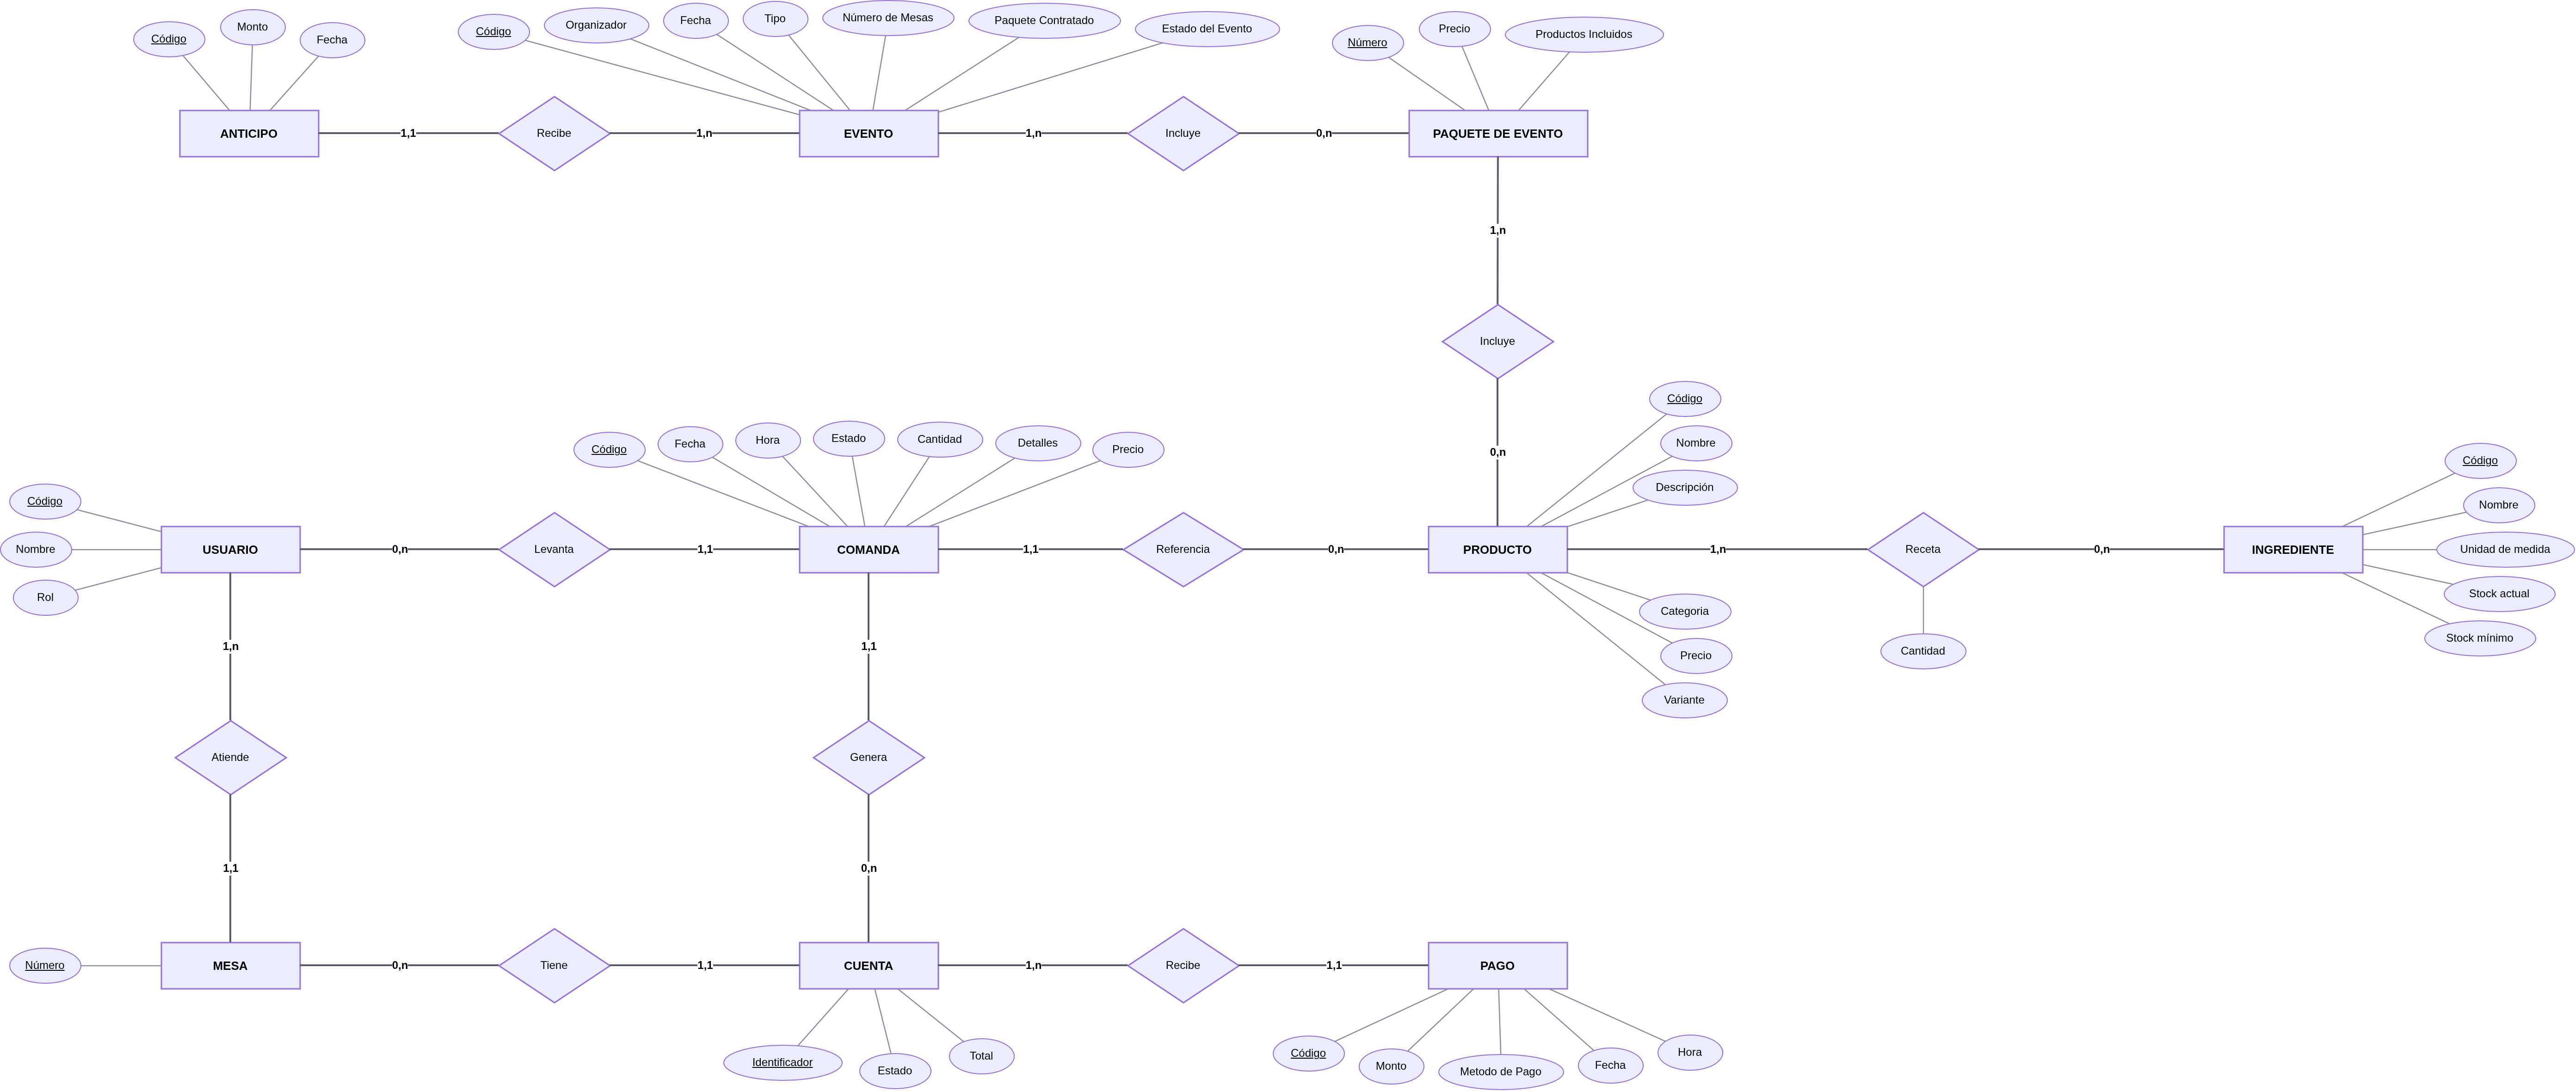
\includegraphics[width=\linewidth, height=0.8\textheight, keepaspectratio]{../../modelo/diagrama-er.png}
        \captionsetup{labelfont=bf, textfont=it, labelsep=newline, justification=raggedright, singlelinecheck=false}
        \caption{Diagrama entidad-relación inicial}
        \label{fig:diagrama-er}
    \end{figure}
    \vspace*{\fill}
\end{paginahorizontal}

\subsection{Limitaciones del modelo básico}

Al revisar de nuevo la entrevista en la Práctica~2, se encontró que el modelo básico obligaba a aplanar o a omitir varias reglas que el cliente sí había mencionado. La Tabla~\ref{tab:er-a-eer} resume esas reglas y el concepto del modelo extendido con el que se representaron.

\begin{table}[H]
    \centering
    \small
    \begin{tabularx}{\textwidth}
        {
            >{\RaggedRight\arraybackslash}X
            >{\RaggedRight\arraybackslash}p{4.2cm}
            >{\RaggedRight\arraybackslash}p{4.2cm}
        }
        \toprule
        \textbf{Regla del negocio} & \textbf{Modelo básico} & \textbf{Modelo extendido} \\
        \midrule
        Los números de mesa y de cuenta se reinician en cada evento. & Mesa y Cuenta con clave propia. & Entidades débiles identificadas por el evento. \\
        Meseros, cocina y bar, y caja guardan datos distintos y realizan funciones distintas. & Un atributo \textit{rol} en Usuario. & Jerarquía de especialización de Usuario. \\
        Ninguna mesa queda sin mesero, pero un mesero puede no tener mesas. & Razón 1:N, sin indicar la obligatoriedad. & Cardinalidades $(\mathit{min}, \mathit{max})$. \\
        Lo acordado de cada producto cambia de un evento a otro aunque sea el mismo paquete. & Solo el contenido general del paquete. & Relación ternaria \textit{Acuerda} con su cantidad. \\
        Un evento puede tener varios organizadores. & Un solo valor por atributo. & Atributo multivaluado. \\
        La fecha y la hora se consultan por día, mes y año. & Campos sueltos. & Atributos compuestos. \\
        \bottomrule
    \end{tabularx}
    \captionsetup{labelfont=bf, textfont=it, labelsep=newline, justification=raggedright, singlelinecheck=false}
    \caption{Reglas que motivaron el modelo extendido}
    \label{tab:er-a-eer}
\end{table}

\subsection{Modelo entidad-relación extendido}

El modelo extendido conserva las entidades del modelo inicial y les agrega los conceptos de la Tabla~\ref{tab:er-a-eer}. Se representó en la notación de Peter Chen, en la que las entidades se dibujan como rectángulos, las relaciones como rombos y los atributos como óvalos; las entidades débiles y sus relaciones identificadoras se distinguen con doble contorno. La Figura~\ref{fig:diagrama-eer} muestra el diagrama completo.

\begin{paginahorizontal}
    \vspace*{\fill}
    \begin{figure}[H]
        \centering
        \includegraphics[width=\linewidth, height=0.8\textheight, keepaspectratio]{../../modelo/diagrama-eer-chen.png}
        \captionsetup{labelfont=bf, textfont=it, labelsep=newline, justification=raggedright, singlelinecheck=false}
        \caption{Diagrama entidad-relación extendido en notación de Peter Chen}
        \label{fig:diagrama-eer}
    \end{figure}
    \vspace*{\fill}
\end{paginahorizontal}

\subsubsection{Entidades débiles}

Mesa y Cuenta son entidades débiles con dependencia de identificación respecto del evento, como se resume en la Tabla~\ref{tab:entidades-debiles}. Decir \enquote{la mesa tres} o \enquote{la cuenta diez} no identifica nada si no se indica el evento, porque la numeración se reinicia en cada uno. Por la misma razón, ninguna de las dos puede existir sin el evento al que pertenece.

\begin{table}[H]
    \centering
    \small
    \begin{tabularx}{\textwidth}
        {
            >{\RaggedRight\arraybackslash}p{2.2cm}
            >{\RaggedRight\arraybackslash}p{2.6cm}
            >{\RaggedRight\arraybackslash}p{3cm}
            >{\RaggedRight\arraybackslash}X
        }
        \toprule
        \textbf{Entidad débil} & \textbf{Propietaria} & \textbf{Clave parcial} & \textbf{Clave completa} \\
        \midrule
        Mesa & Evento & Número de mesa & (Número de evento, Número de mesa) \\
        Cuenta & Evento & Secuencial & (Número de evento, Secuencial) \\
        \bottomrule
    \end{tabularx}
    \captionsetup{labelfont=bf, textfont=it, labelsep=newline, justification=raggedright, singlelinecheck=false}
    \caption{Entidades débiles del modelo}
    \label{tab:entidades-debiles}
\end{table}

\subsubsection{Jerarquía de Usuario}

Usuario se especializa en tres subclases: Mesero, Bar/Cocina y Cajero/Administrador. La especialización se justifica porque cada subclase tiene atributos propios, como el turno del mesero o la estación asignada de la cocina o el bar, y sobre todo relaciones propias: el mesero atiende mesas y levanta comandas, la cocina y el bar preparan comandas, y el cajero maneja pagos y cancela comandas. Si solo cambiaran los atributos, un campo de rol habría bastado.

La especialización es \textbf{disjunta}, porque una persona desempeña un solo puesto a la vez, y esa separación es la que da sentido al control que pidió el cliente: quien cobra no puede ser quien recibe la propina de ese cobro, y quien cancela una comanda no puede ser quien la levantó. Es además \textbf{total}, porque todo usuario del sistema es personal del salón y tiene un puesto; el organizador del evento no es usuario, sino un dato del evento. La cocina y el bar se agruparon en una sola subclase porque tienen los mismos atributos y la misma función, y su estación asignada indica cuál es cuál.

\subsubsection{Relaciones y cardinalidades}

Las cardinalidades se expresaron con la notación $(\mathit{min}, \mathit{max})$, que indica para cada entidad con cuántas instancias de la otra se asocia como mínimo y como máximo. La Tabla~\ref{tab:relaciones} reúne las diecisiete relaciones del modelo; en cada par, la primera cardinalidad corresponde a la primera entidad.

\begin{table}[H]
    \centering
    \footnotesize
    \begin{tabularx}{\textwidth}
        {
            >{\RaggedRight\arraybackslash}p{3.2cm}
            >{\RaggedRight\arraybackslash}p{4.6cm}
            >{\RaggedRight\arraybackslash}p{2.4cm}
            >{\RaggedRight\arraybackslash}X
        }
        \toprule
        \textbf{Relación} & \textbf{Entidades} & \textbf{Cardinalidad} & \textbf{Regla} \\
        \midrule
        \textit{Pertenece} (identificadora) & Mesa -- Evento & (1,1):(1,N) & Toda mesa es de un evento y todo evento tiene mesas. \\
        \textit{Abre} (identificadora) & Evento -- Cuenta & (0,N):(1,1) & Toda cuenta se abre en un evento. \\
        \textit{Atiende} & Mesa -- Mesero & (1,1):(0,N) & Ninguna mesa queda sin mesero. \\
        \textit{Tiene} & Mesa -- Cuenta & (0,N):(1,1) & Una mesa tiene varias cuentas. \\
        \textit{Genera} & Cuenta -- Comanda & (0,N):(1,1) & Una cuenta pide varias rondas. \\
        \textit{Levanta} & Mesero -- Comanda & (0,N):(1,1) & Cada comanda tiene un mesero responsable. \\
        \textit{Prepara} & Bar/Cocina -- Comanda & (0,N):(0,1) & Una comanda pendiente aún no tiene estación. \\
        \textit{Cancela} & Cajero -- Comanda & (0,N):(0,1) & Solo caja cancela comandas. \\
        \textit{Referencia} & Comanda -- Producto & (1,1):(0,N) & Cada comanda pide un producto. \\
        \textit{Variante} & Producto -- Producto & (0,N):(0,1) & Una variante tiene un solo producto principal. \\
        \textit{Receta} & Producto -- Ingrediente & (1,N):(0,N) & Todo producto lleva al menos un ingrediente. \\
        \textit{Incluye} & Paquete -- Producto & (1,N):(0,N) & Contenido base de cada paquete. \\
        \textit{Acuerda} (ternaria) & Evento -- Paquete -- Producto & (0,N) en cada una & Lo pactado para cada evento. \\
        \textit{Recibe} & Evento -- Anticipo & (0,N):(1,1) & Los anticipos son del evento. \\
        \textit{Recibe} & Cuenta -- Pago & (0,N):(1,1) & Una cuenta puede pagarse en partes. \\
        \textit{Maneja} & Cajero -- Pago & (0,N):(1,1) & Cada pago lo registra un cajero. \\
        \textit{Recibe propina} & Mesero -- Pago & (0,N):(0,1) & Un pago puede dejar propina a un mesero. \\
        \bottomrule
    \end{tabularx}
    \captionsetup{labelfont=bf, textfont=it, labelsep=newline, justification=raggedright, singlelinecheck=false}
    \caption{Relaciones del modelo entidad-relación extendido}
    \label{tab:relaciones}
\end{table}

\subsubsection{Relación ternaria y atributos de relación}

Una relación entre tres entidades solo se justifica cuando ninguna de ellas queda determinada por las otras dos. \textit{Acuerda} cumple esa condición: si un evento contrata dos paquetes que incluyen el mismo producto, conocer el evento y el producto no indica cuánto se acordó por cada paquete, por lo que se necesitan las tres entidades. En cambio, \textit{Prepara} se mantuvo binaria, porque cada comanda apunta a un solo producto y agregarlo a la relación no aportaba información.

Tres datos no pertenecen a ninguna entidad, sino a la relación que las une: la \textit{cantidad acordada} de \textit{Acuerda}, base de la comparación entre lo presupuestado y lo consumido; la \textit{cantidad por porción} de \textit{Receta}, con la que se descuenta el inventario al preparar cada comanda; y el \textit{monto de propina} de \textit{Recibe propina}, que corresponde a un cobro concreto y no al mesero ni al pago por separado.

\subsubsection{Atributos especiales}

El modelo incluye un atributo multivaluado, los organizadores del evento, y atributos compuestos para la fecha y la hora, que se consultan por sus componentes. También identifica atributos derivados, cuyo valor se calcula a partir de otros datos y no se captura: el total acumulado de cada cuenta, las propinas acumuladas de cada mesero, la edad de cada usuario, el número de mesas de cada evento y la disponibilidad de cada producto, que depende de que todos los ingredientes de su receta alcancen para una porción.

\subsection{Restricciones que el diagrama no expresa}

Un diagrama entidad-relación no puede representar todas las reglas del negocio. Las siguientes quedaron documentadas junto al modelo para resolverse en la implementación:

\begin{itemize}
    \item El total acumulado de una cuenta debe coincidir con la suma de sus comandas.
    \item El precio cobrado se copia del catálogo al levantar la comanda y no cambia aunque después cambie el precio del producto.
    \item Solo el cajero o administrador puede cancelar comandas.
    \item Al preparar una comanda se descuenta del inventario la cantidad por porción de cada ingrediente, y la existencia nunca puede quedar negativa.
    \item El rol que se guarda es el actual: si un mesero pasa a caja, las comandas y los pagos que ya registró conservan su autoría.
    \item El contenido de un paquete es una base y no una lista cerrada, por lo que en un evento pueden acordarse productos o cantidades distintos de los del catálogo.
\end{itemize}

La sección de implementación describe cómo cada una de estas reglas se convirtió en una restricción, un disparador o una vista del esquema.


	% Diseño lógico
	\newpage

\section{Diseño lógico}
\label{sec:diseno-logico}

En esta sección se describe la transformación del modelo entidad-relación extendido en un esquema relacional, trabajada en la Práctica~3. Se presentan el inventario del que partió la transformación, las decisiones de tipos de dato, la forma en que se aplicó cada regla, el esquema resultante y la revisión de que este conserva el significado del modelo.

\subsection{Inventario del modelo extendido}

Antes de aplicar las reglas se levantó un inventario de los elementos del modelo extendido, porque cada tipo de elemento se transforma con una regla distinta y omitir uno habría dejado una parte del negocio sin representar. La Tabla~\ref{tab:inventario} resume ese inventario.

\begin{table}[H]
    \centering
    \small
    \begin{tabular}{lc}
        \toprule
        \textbf{Elemento} & \textbf{Cantidad} \\
        \midrule
        Entidades fuertes & 8 \\
        Entidades débiles & 2 \\
        Subclases de la jerarquía de Usuario & 3 \\
        Relaciones binarias uno a muchos & 14 \\
        Relaciones binarias muchos a muchos & 2 \\
        Relaciones ternarias & 1 \\
        Atributos multivaluados & 1 \\
        Atributos compuestos & 5 \\
        Atributos derivados & 7 \\
        Atributos de relación & 3 \\
        \bottomrule
    \end{tabular}
    \captionsetup{labelfont=bf, textfont=it, labelsep=newline, justification=raggedright, singlelinecheck=false}
    \caption{Inventario del modelo entidad-relación extendido}
    \label{tab:inventario}
\end{table}

\subsection{Tipos de dato}

Para no justificar cada columna por separado, se fijó primero el tipo que recibe cada clase de atributo, como se muestra en la Tabla~\ref{tab:tipos}. El criterio general fue elegir el tipo que valida el dato por sí mismo: un tipo de fecha rechaza el 31 de febrero y un decimal exacto evita que las sumas de dinero acumulen errores de redondeo, como ocurriría con los tipos de punto flotante.

\begin{table}[H]
    \centering
    \small
    \begin{tabularx}{\textwidth}
        {
            >{\RaggedRight\arraybackslash}p{3.6cm}
            >{\RaggedRight\arraybackslash}p{4.2cm}
            >{\RaggedRight\arraybackslash}X
        }
        \toprule
        \textbf{Clase de atributo} & \textbf{Tipo en PostgreSQL} & \textbf{Razón} \\
        \midrule
        Identificadores & \texttt{INTEGER} con identidad & El gestor asigna el siguiente número y permite cargar números conocidos. \\
        Claves parciales & \texttt{SMALLINT} & Se reinician en cada evento y nunca son grandes. \\
        Dinero & \texttt{NUMERIC(10,2)} & Decimal exacto a centavos. \\
        Cantidades de inventario & \texttt{NUMERIC(10,3)} & Decimal exacto en gramos, mililitros o piezas. \\
        Listas cerradas & \texttt{VARCHAR} con \texttt{CHECK} & La lista queda visible y puede ampliarse. \\
        Fechas e instantes & \texttt{DATE} y \texttt{TIMESTAMPTZ} & Validan la fecha y guardan el instante exacto. \\
        Contraseñas & \texttt{VARCHAR(255)} & Solo se guarda su \textit{hash}, nunca el texto. \\
        \bottomrule
    \end{tabularx}
    \captionsetup{labelfont=bf, textfont=it, labelsep=newline, justification=raggedright, singlelinecheck=false}
    \caption{Tipos de dato por clase de atributo}
    \label{tab:tipos}
\end{table}

\subsection{Aplicación de las reglas de transformación}

La transformación siguió las nueve reglas descritas en el marco teórico \parencite[p.~289]{elmasri_navathe}. En algunos casos fue necesario interpretar la regla para no perder una propiedad del modelo; esas decisiones se explican a continuación.

\subsubsection{Entidades, atributos compuestos y multivaluados}

Las ocho entidades fuertes produjeron ocho tablas, cada una con su identificador como clave primaria. Los cinco atributos compuestos son todos de fecha u hora, y el cliente los consulta por sus componentes; aplicar la regla al pie de la letra, guardando el día, el mes y el año como columnas sueltas, habría permitido guardar fechas imposibles. Por ello, la fecha se guarda con el tipo nativo del gestor, que la valida, y cada componente es una columna generada que el gestor calcula y que nadie puede escribir, de modo que nunca contradice a la fecha. El único atributo multivaluado, los organizadores del evento, se llevó a una tabla propia cuya clave combina el evento y el organizador.

Los atributos derivados no se guardan, porque una copia de un dato calculado debe mantenerse sincronizada y, si alguna vez no se actualiza, la base tiene dos versiones distintas de lo mismo. En su lugar, se calculan en vistas: el número de mesas del evento, el total acumulado y el saldo de cada cuenta, la edad de cada usuario, las propinas acumuladas de cada mesero y la disponibilidad de cada producto. El precio cobrado de una comanda, en cambio, sí se guarda, porque es el precio que tenía el producto al momento del pedido y no debe cambiar aunque el catálogo cambie después.

\subsubsection{Relaciones}

Las catorce relaciones uno a muchos se representaron con una clave foránea en la tabla del lado de muchos, y su participación mínima se expresó con \texttt{NOT NULL} cuando es obligatoria. Las dos relaciones muchos a muchos, \textit{Receta} e \textit{Incluye}, produjeron las tablas \texttt{receta} y \texttt{paquete\_producto}, cuyas claves combinan las de las dos entidades y que conservan los atributos de la relación, como la cantidad por porción.

La relación ternaria \textit{Acuerda} produjo la tabla \texttt{acuerdo}, cuya clave primaria combina las claves del evento, del paquete y del producto, porque ningún par de ellas determina al tercero. Esta tabla no tiene una clave foránea hacia \texttt{paquete\_producto}: el contenido del paquete es una base y no una lista cerrada, y esa clave haría que el gestor rechazara justamente lo que el negocio permite, acordar en un evento un producto que el paquete no traía.

\subsubsection{Entidades débiles}

Mesa y Cuenta dependen del evento por identificación, así que sus tablas llevan una clave primaria compuesta por el número de evento y su clave parcial. De esta forma, la mesa tres de un evento y la de otro son filas distintas, y el gestor rechaza una segunda mesa tres en el mismo evento. Su clave foránea hacia el evento borra en cascada, porque una mesa o una cuenta no tienen sentido sin su evento; sin embargo, esa cascada se detiene si el evento ya tiene comandas, pagos o anticipos, cuyas claves impiden el borrado para conservar el historial del dinero.

\subsubsection{Jerarquía de Usuario}

Para la jerarquía se eligió la estrategia de una tabla para la superclase y una para cada subclase. Aunque las subclases tienen pocos atributos propios, lo que decidió la estrategia fueron sus relaciones: seis relaciones solo admiten a usuarios de una subclase, como la propina, que solo puede ir a un mesero, y eso exige que la clave foránea apunte a la tabla \texttt{mesero} y no a \texttt{usuario}. Con una sola tabla para toda la jerarquía, el gestor aceptaría una propina para un cocinero; y sin la tabla de la superclase, los datos comunes se repetirían en tres tablas y el nombre de acceso no podría ser único entre todas ellas.

La restricción disjunta se hace cumplir de forma declarativa: la tabla \texttt{usuario} guarda un discriminador \texttt{rol}, cada subclase lo repite fijo a su valor y apunta a \texttt{usuario} con una clave foránea de dos columnas, el identificador y el rol, de modo que un usuario no puede aparecer en dos subclases. La restricción total se verifica con un disparador diferido que, al confirmar la transacción, comprueba que cada usuario tenga su fila en la subclase que corresponde a su rol.

\subsection{Esquema resultante}

La transformación produjo diecisiete tablas y seis vistas, que se listan en la Tabla~\ref{tab:tablas} junto con el elemento del modelo del que provienen. La Figura~\ref{fig:diagrama-relacional} muestra el diagrama relacional, en el que se distinguen la clave primaria, las claves foráneas y las columnas generadas de cada tabla.

\begin{table}[H]
    \centering
    \small
    \begin{tabularx}{\textwidth}
        {
            >{\RaggedRight\arraybackslash}p{3.4cm}
            >{\RaggedRight\arraybackslash}X
        }
        \toprule
        \textbf{Tabla} & \textbf{Origen en el modelo extendido} \\
        \midrule
        \texttt{evento} & Entidad fuerte Evento \\
        \texttt{evento\_organizador} & Atributo multivaluado de Evento \\
        \texttt{usuario} & Superclase Usuario \\
        \texttt{mesero}, \texttt{bar\_cocina}, \texttt{cajero\_admin} & Subclases de Usuario \\
        \texttt{mesa}, \texttt{cuenta} & Entidades débiles, con las relaciones \textit{Atiende} y \textit{Tiene} \\
        \texttt{producto} & Entidad fuerte Producto, con la relación \textit{Variante} \\
        \texttt{ingrediente}, \texttt{paquete} & Entidades fuertes \\
        \texttt{receta}, \texttt{paquete\_producto} & Relaciones muchos a muchos \textit{Receta} e \textit{Incluye} \\
        \texttt{acuerdo} & Relación ternaria \textit{Acuerda} \\
        \texttt{comanda} & Entidad fuerte Comanda, con \textit{Genera}, \textit{Levanta}, \textit{Referencia}, \textit{Prepara} y \textit{Cancela} \\
        \texttt{pago} & Entidad fuerte Pago, con \textit{Recibe}, \textit{Maneja} y \textit{Recibe propina} \\
        \texttt{anticipo} & Entidad fuerte Anticipo, con \textit{Recibe} \\
        \bottomrule
    \end{tabularx}
    \captionsetup{labelfont=bf, textfont=it, labelsep=newline, justification=raggedright, singlelinecheck=false}
    \caption{Tablas del esquema relacional}
    \label{tab:tablas}
\end{table}

\begin{figure}[p]
    \centering
    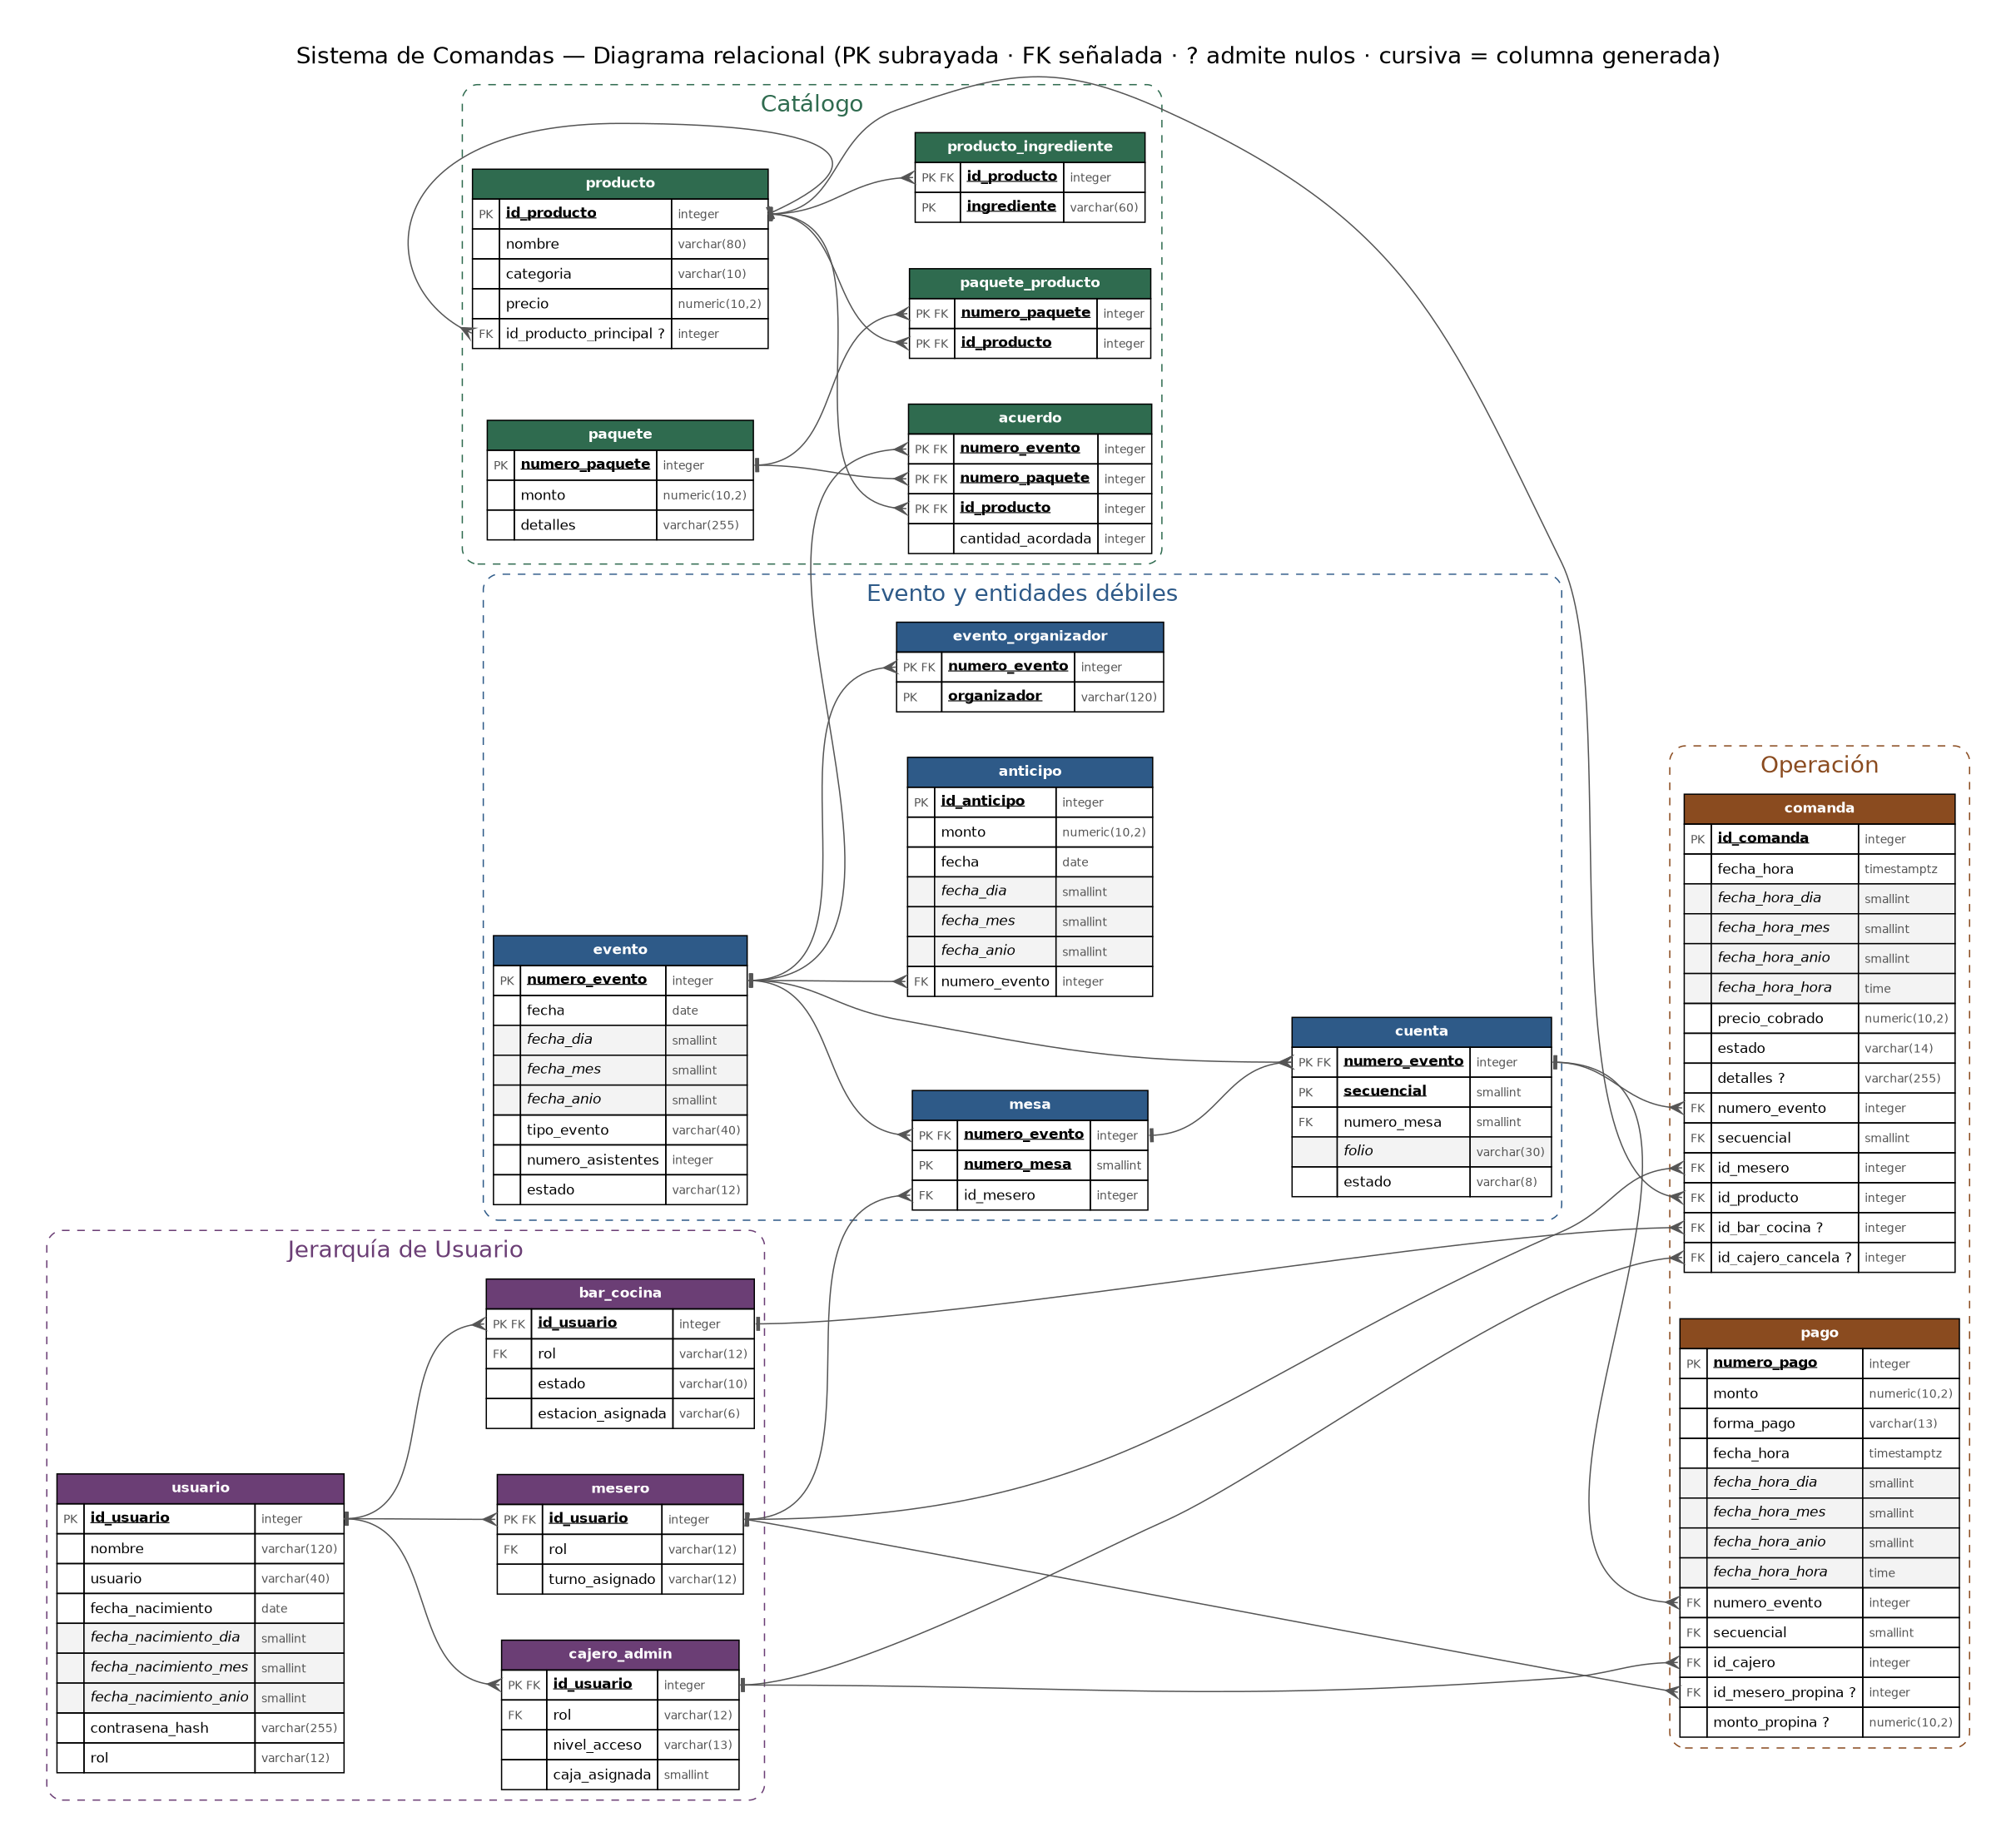
\includegraphics[width=\linewidth, height=0.85\textheight, keepaspectratio]{../../modelo/diagrama-relacional.png}
    \captionsetup{labelfont=bf, textfont=it, labelsep=newline, justification=raggedright, singlelinecheck=false}
    \caption{Diagrama relacional del sistema de comandas}
    \label{fig:diagrama-relacional}
\end{figure}

En total, el esquema tiene noventa y siete columnas y veinticinco claves foráneas. El diccionario de datos, con el tipo, las restricciones y la descripción de cada columna, se encuentra en el repositorio del proyecto.

\subsection{Preservación del significado}

Una vez ejecutado el esquema, se revisó contra el inventario, elemento por elemento, que conservara el significado del modelo extendido. Las ocho entidades fuertes, las dos débiles y las tres subclases tienen su tabla, y cada relación quedó expresada con restricciones: el máximo de uno, en la tabla donde vive la clave foránea; el máximo de muchos, en que esa columna no es única; y el mínimo, en que la columna sea obligatoria o admita nulos.

Algunas reglas no se hacen cumplir en el esquema, y se dejaron documentadas para que las valide la aplicación. Que todo evento tenga al menos una mesa y todo producto al menos un ingrediente no se exige, porque el evento se registra semanas antes de montar las mesas y la receta se captura después de dar de alta el producto; el número máximo de mesas depende del acomodo del salón; y que el mesero que recibe la propina sea quien atendió la mesa no es una regla, porque un mesero puede cubrir a otro.

La única regla del modelo extendido que no se preservó es el cambio de rol conservando el historial. Como la clave foránea de cada subclase incluye el rol, el gestor impide cambiar el rol de un usuario que ya tiene registros, de modo que el historial queda protegido, pero el cambio de puesto requiere un procedimiento administrativo. Se aceptó esta limitación porque la disyunción es la regla que sostiene el control del dinero y el cambio de rol es un evento poco frecuente; si llegara a ser común, la solución sería separar la identidad de la persona del rol que desempeña en cada periodo.


	% Implementación
	\newpage

\section{Implementación}
\label{sec:implementacion}

En esta sección se describe la implementación física del esquema en PostgreSQL: su ejecución y la forma en que se modificó después, los tipos y dominios, las restricciones de columna, los disparadores y las vistas que hacen cumplir las reglas del negocio, los roles con los que se accede a la base y las pruebas con las que se comprobó cada restricción. Este trabajo se realizó en las prácticas~3 y~4.

\subsection{Ejecución del esquema y migraciones}

El esquema relacional se escribió en un solo script de definición de datos que crea las diecisiete tablas, sus restricciones, los disparadores, las vistas y un comentario en cada tabla y columna, que el gestor guarda en su catálogo como parte del diccionario de datos. El script se ejecutó sobre una base vacía dentro del contenedor descrito en la metodología, junto con un conjunto pequeño de datos de ejemplo con el que se probaron las restricciones.

A partir de la Práctica~4, el script original ya no se editó: cada cambio posterior al esquema se escribió como una migración numerada con sentencias \texttt{ALTER TABLE}, que se aplica después del script y en orden. Así, cualquier base puede llevarse al estado actual ejecutando el script y las migraciones, y la historia de los cambios queda registrada. La Tabla~\ref{tab:migraciones} resume las migraciones del proyecto.

\begin{table}[H]
    \centering
    \small
    \begin{tabularx}{\textwidth}
        {
            >{\RaggedRight\arraybackslash}p{4.4cm}
            >{\RaggedRight\arraybackslash}X
        }
        \toprule
        \textbf{Migración} & \textbf{Cambio} \\
        \midrule
        \texttt{001-dominios.sql} & Crea los dominios \texttt{dinero} y \texttt{cantidad} y cambia a ellos las columnas de importes y de inventario. \\
        \texttt{002-formato-usuario.sql} & Agrega la restricción de formato del nombre de acceso de los usuarios. \\
        \texttt{099-permisos.sql} & Crea los roles de la aplicación, de consulta y de administración, y les otorga sus permisos. \\
        \bottomrule
    \end{tabularx}
    \captionsetup{labelfont=bf, textfont=it, labelsep=newline, justification=raggedright, singlelinecheck=false}
    \caption{Migraciones aplicadas al esquema}
    \label{tab:migraciones}
\end{table}

La migración de permisos lleva el número 99 para ejecutarse siempre al final, de modo que alcance a las tablas o columnas que agreguen las migraciones anteriores.

\subsection{Tipos de dato y dominios}

Cada una de las noventa y siete columnas recibió el tipo y la precisión justificados en el diseño lógico. Ninguna columna usa punto flotante: los importes son decimales exactos a centavos, las cantidades de inventario son decimales exactos a milésimas, las fechas usan los tipos nativos del gestor y los identificadores son enteros que el gestor asigna con una secuencia.

Los importes aparecen en seis columnas de cinco tablas, y las cantidades de inventario en tres columnas de dos tablas. Para no repetir su tipo y su precisión en cada una, se definieron dos dominios con la sentencia \texttt{CREATE DOMAIN} \parencite{postgres_createdomain}, como se muestra en el Código~\ref{cod:dominios}. Con ellos, todas las columnas de dinero comparten exactamente la misma definición, y si en el futuro cambiara la precisión, bastaría con modificar el dominio. Las reglas propias de cada columna, como que un precio no sea negativo, se mantuvieron en sus restricciones \texttt{CHECK}, porque no son iguales en todas.

\begin{lstlisting}[style=codigoC, language=SQL, caption={Dominios de la migración \texttt{001-dominios.sql}}, label=cod:dominios]
CREATE DOMAIN dinero AS NUMERIC(10,2);
CREATE DOMAIN cantidad AS NUMERIC(10,3);

ALTER TABLE producto
    ALTER COLUMN precio TYPE dinero USING precio::dinero;
\end{lstlisting}

\subsection{Restricciones de columna}

Las restricciones de columna hacen cumplir las reglas que dependen de una sola fila \parencite{postgres_constraints}. El esquema declara las siguientes:

\begin{itemize}
    \item \textbf{\texttt{NOT NULL}} en todo atributo sin el cual la fila no tiene sentido y en veintiuna de las veinticinco claves foráneas. Las otras cuatro admiten nulos porque su participación mínima es cero: el producto principal de una variante, la estación que prepara una comanda, el cajero que la canceló y el mesero que recibe la propina.
    \item \textbf{\texttt{DEFAULT}} en trece columnas con un valor inicial natural, como el estado inicial de un evento o de una comanda, la fecha y hora actual o una existencia de cero.
    \item \textbf{\texttt{UNIQUE}} en cuatro columnas o combinaciones, y tres índices únicos para reglas que una restricción simple no expresa: los nombres de acceso y los nombres de ingredientes no pueden repetirse aunque cambien las mayúsculas, y dos cuentas abiertas de una misma mesa no pueden llamarse igual.
    \item \textbf{\texttt{CHECK}} en treinta y seis reglas de rango, de lista de valores, de formato y entre columnas. La Tabla~\ref{tab:check} muestra ejemplos de cada tipo.
\end{itemize}

\begin{table}[H]
    \centering
    \small
    \begin{tabularx}{\textwidth}
        {
            >{\RaggedRight\arraybackslash}p{2.4cm}
            >{\RaggedRight\arraybackslash}p{5.4cm}
            >{\RaggedRight\arraybackslash}X
        }
        \toprule
        \textbf{Tipo} & \textbf{Restricción} & \textbf{Regla del negocio} \\
        \midrule
        Rango & \texttt{ck\_ingrediente\_stock} & Las existencias de un ingrediente nunca son negativas. \\
        Lista de valores & \texttt{ck\_comanda\_estado} & Una comanda solo puede estar pendiente, en preparación, lista, entregada o cancelada. \\
        Formato & \texttt{ck\_usuario\_formato} & El nombre de acceso empieza con una letra y solo lleva letras y números, de 3 a 40 caracteres. \\
        Entre columnas & \texttt{ck\_pago\_propina\_limite} & La propina no puede superar el monto pagado. \\
        Entre columnas & \texttt{ck\_comanda\_cancelacion} & Una comanda está cancelada si y solo si registra al cajero que la canceló. \\
        \bottomrule
    \end{tabularx}
    \captionsetup{labelfont=bf, textfont=it, labelsep=newline, justification=raggedright, singlelinecheck=false}
    \caption{Ejemplos de restricciones \texttt{CHECK}}
    \label{tab:check}
\end{table}

\subsection{Reglas del negocio con disparadores}

Las reglas que relacionan varias filas o varias tablas no pueden expresarse con una restricción de columna, por lo que se implementaron con disparadores \parencite{postgres_triggers}. La Tabla~\ref{tab:disparadores} relaciona cada regla del negocio enunciada en el caso de estudio con el disparador que la hace cumplir.

\begin{table}[H]
    \centering
    \small
    \begin{tabularx}{\textwidth}
        {
            >{\RaggedRight\arraybackslash}X
            >{\RaggedRight\arraybackslash}p{5cm}
        }
        \toprule
        \textbf{Regla del negocio} & \textbf{Disparador} \\
        \midrule
        El precio cobrado se copia del catálogo y no puede modificarse después. & \texttt{tg\_comanda\_precio} \\
        Una comanda solo avanza de estado y una cancelada ya no cambia. & \texttt{tg\_comanda\_estado} \\
        Cada comanda la prepara la estación de su categoría. & \texttt{tg\_comanda\_estacion} \\
        No se levantan comandas en un evento finalizado. & \texttt{tg\_comanda\_evento} \\
        No se levantan comandas en una cuenta cerrada. & \texttt{tg\_comanda\_cuenta\_abierta} \\
        Al preparar una comanda se descuenta la receta del inventario. & \texttt{tg\_comanda\_stock} \\
        Un pago no puede exceder el saldo de la cuenta. & \texttt{tg\_pago\_saldo} \\
        Una cuenta solo se cierra sin adeudo y con sus comandas terminadas. & \texttt{tg\_cuenta\_cierre} \\
        Una variante no puede tener variantes. & \texttt{tg\_producto\_variante} \\
        Todo usuario pertenece a la subclase de su rol. & \texttt{ct\_usuario\_total} y uno por subclase \\
        \bottomrule
    \end{tabularx}
    \captionsetup{labelfont=bf, textfont=it, labelsep=newline, justification=raggedright, singlelinecheck=false}
    \caption{Reglas del negocio implementadas con disparadores}
    \label{tab:disparadores}
\end{table}

El descuento de inventario ocurre una sola vez, cuando la comanda pasa por primera vez a preparación, y si algún ingrediente no alcanza, el disparador rechaza la operación con un mensaje que indica cuánto queda y cuánto pide la receta. Los disparadores de la especialización total son diferidos: se revisan al confirmar la transacción, lo que permite insertar primero al usuario y después su fila de subclase.

El Código~\ref{cod:pago-saldo} muestra la función del disparador que protege el cobro. Antes de comparar, bloquea la fila de la cuenta con \texttt{FOR UPDATE}, de modo que dos cajeros que registren pagos a la misma cuenta al mismo tiempo no puedan exceder el saldo entre los dos: el segundo pago espera a que el primero termine y se compara contra el saldo ya actualizado.

\begin{lstlisting}[style=codigoC, language=SQL, caption={Función del disparador \texttt{tg\_pago\_saldo}}, label=cod:pago-saldo, morekeywords={RETURNS, LANGUAGE, PERFORM, RAISE, EXCEPTION, USING, ERRCODE, RETURN, NEW, COALESCE, DECLARE}]
CREATE FUNCTION validar_pago_saldo() RETURNS trigger
LANGUAGE plpgsql AS $$
DECLARE
    v_saldo NUMERIC(10,2);
BEGIN
    PERFORM 1 FROM cuenta
    WHERE numero_evento = NEW.numero_evento AND secuencial = NEW.secuencial
    FOR UPDATE;
    SELECT saldo INTO v_saldo FROM v_cuenta
    WHERE numero_evento = NEW.numero_evento AND secuencial = NEW.secuencial;
    IF NEW.monto - COALESCE(NEW.monto_propina, 0) > v_saldo THEN
        RAISE EXCEPTION 'el pago excede el saldo de la cuenta (%)', v_saldo
            USING ERRCODE = 'check_violation';
    END IF;
    RETURN NEW;
END;
$$;
\end{lstlisting}

\subsection{Vistas}

Los atributos derivados del modelo se calculan en seis vistas \parencite{postgres_createview}, una por cada tabla que los requiere. La más importante para la operación es \texttt{v\_cuenta}, que calcula para cada cuenta el total acumulado de sus comandas no canceladas, el total pagado sin contar las propinas y el saldo pendiente; tanto el disparador del cobro como el del cierre de cuenta consultan esta vista, de modo que la regla y el reporte usan exactamente el mismo cálculo. Las demás vistas calculan el número de mesas de cada evento, la edad de cada usuario, las propinas acumuladas de cada mesero, el precio vigente del producto de cada comanda y la disponibilidad de cada producto según su receta y el inventario.

\subsection{Usuarios y permisos}

Una base que siempre se usa con el usuario administrador no está protegida, porque cualquier error de un programa podría borrar o modificar cualquier dato. Por ello se definieron tres roles con el principio de mínimo privilegio \parencites{postgres_roles}{postgres_privileges}, cada uno con un usuario que solo hereda sus permisos y cuya contraseña se toma de variables de entorno. La Tabla~\ref{tab:roles} los resume, y la matriz con los privilegios de cada rol sobre cada tabla y vista se encuentra en el \hyperref[anexo:permisos]{Anexo~2}.

\begin{table}[H]
    \centering
    \small
    \begin{tabularx}{\textwidth}
        {
            >{\RaggedRight\arraybackslash}p{3.2cm}
            >{\RaggedRight\arraybackslash}X
        }
        \toprule
        \textbf{Rol} & \textbf{Para qué existe y qué puede hacer} \\
        \midrule
        \texttt{comandas\_app} & Lo usan el servidor del sistema y el script de carga. Opera el salón, pero no puede borrar comandas, eventos, mesas ni cuentas, porque estos cambian de estado en lugar de borrarse; solo puede insertar pagos y anticipos, nunca modificarlos; y no puede alterar la estructura. \\
        \texttt{comandas\_consulta} & Para reportes. Solo lee, y no puede ver el \textit{hash} de las contraseñas, porque su permiso sobre la tabla de usuarios se otorgó columna por columna. \\
        \texttt{comandas\_admin} & Para correcciones manuales. Puede leer y modificar todas las tablas, pero no es su dueño, así que no puede borrarlas ni crear roles. \\
        \bottomrule
    \end{tabularx}
    \captionsetup{labelfont=bf, textfont=it, labelsep=newline, justification=raggedright, singlelinecheck=false}
    \caption{Roles de la base de datos}
    \label{tab:roles}
\end{table}

Los disparadores se ejecutan con los permisos de quien realiza la operación, de modo que levantar una comanda requiere, además del permiso de inserción, poder bloquear la cuenta, consultar el evento y descontar el inventario. Se optó por conceder esos permisos al rol de la aplicación, que de todos modos los necesita para cerrar cuentas, cambiar el estado de los eventos y resurtir ingredientes, en lugar de declarar las funciones con los privilegios de su dueño, lo que no habría aportado ninguna protección.

Cada rol se probó con operaciones permitidas y negadas, y en todos los casos el gestor respondió como se esperaba; por ejemplo, borrar una comanda con el rol de la aplicación produce el error \texttt{permission denied for table comanda}. También se comprobó que al retirar un permiso con \texttt{REVOKE} la operación deja de funcionar, y que vuelve a funcionar al devolverlo con \texttt{GRANT}.

\subsection{Pruebas de las restricciones}

Cada restricción del esquema se comprobó con una instrucción diseñada para violarla, y cada regla con un caso válido que debe aceptarse. El conjunto de pruebas reúne treinta y seis instrucciones que el gestor debe rechazar y quince casos válidos que debe aceptar, y se ejecuta con un solo comando que se detiene si alguna prueba no da el resultado esperado. Entre ellas, diez casos documentan con detalle las restricciones de dominio: \texttt{NOT NULL}, \texttt{DEFAULT}, \texttt{UNIQUE} simple y compuesta, y \texttt{CHECK} de rango, de formato y entre columnas, cada uno con la operación intentada, el mensaje del gestor y la regla protegida. En la última ejecución, las treinta y seis instrucciones fueron rechazadas y los quince casos válidos se aceptaron.


	% Población de la base de datos
	\newpage

\section{Población de la base de datos}
\label{sec:poblacion}

En esta sección se describe cómo se obtuvieron los datos con los que se pobló la base y el script con el que se cargan. Este trabajo corresponde a la Práctica~4, cuyo requisito era contar con al menos doscientos renglones en cada tabla principal, provenientes de una fuente documentada y cargados con un solo comando.

\subsection{Búsqueda de una fuente de datos}

Las tablas de la base se dividen en dos grupos con necesidades distintas: el catálogo, formado por los productos, los ingredientes y las recetas, requiere platillos y bebidas con las cantidades de sus ingredientes; la operación, formada por los eventos, las mesas, las cuentas, las comandas, los pagos y los anticipos, requiere pedidos registrados uno por uno, con su mesa, su mesero, su estado y su pago.

Para cada grupo se buscaron conjuntos de datos publicados en los portales de datos abiertos de la Ciudad de México y del gobierno federal, en el repositorio DataMX y en buscadores generales, con términos como \textit{comandas}, \textit{recetas}, \textit{restaurantes} y \textit{banquetes}. Para la operación no se encontró ningún conjunto con pedidos de un salón de eventos: los resultados eran directorios de negocios, estadísticas agregadas o conjuntos de pedidos declarados como ficticios por sus propios autores. El resultado es razonable, porque los pedidos son datos internos de cada negocio y contienen información de sus clientes y empleados. Para el catálogo, el único conjunto que ofrecía recetas con cantidades y una licencia que permite su uso fue la base de datos de alimentos y nutrientes del Departamento de Agricultura de los Estados Unidos \parencite{usda_fndds}, publicada en el dominio público.

\subsection{Fuente elegida}

Siguiendo el orden que pide la práctica, los datos se buscaron primero en el propio caso de estudio. El salón de eventos permitió publicar su menú vigente \parencite{menu_salon}, pero no cuenta con recetas fijas ni con registros de pedidos que compartir. Por ello, cada tabla se pobló con la mejor fuente disponible, como se resume en la Tabla~\ref{tab:fuentes}.

\begin{table}[H]
    \centering
    \small
    \begin{tabularx}{\textwidth}
        {
            >{\RaggedRight\arraybackslash}X
            >{\RaggedRight\arraybackslash}X
            >{\RaggedRight\arraybackslash}p{2cm}
        }
        \toprule
        \textbf{Datos} & \textbf{Origen} & \textbf{Tipo} \\
        \midrule
        122 de los 214 productos & Menú del salón y variantes confirmadas por un integrante que trabajó en él & Reales \\
        85 de los 208 ingredientes y 292 de las 681 filas de receta & Estimados a partir del menú, con las proporciones de FNDDS donde el platillo coincide & Estimados \\
        92 productos y 123 ingredientes con sus recetas & Script de generación, para superar los doscientos renglones & Inventados \\
        Usuarios, eventos, mesas, cuentas, comandas, pagos, anticipos y paquetes & Script de generación con semilla fija & Sintéticos \\
        \bottomrule
    \end{tabularx}
    \captionsetup{labelfont=bf, textfont=it, labelsep=newline, justification=raggedright, singlelinecheck=false}
    \caption{Origen de los datos de cada tabla}
    \label{tab:fuentes}
\end{table}

\subsubsection{Menú del salón}

El menú se obtuvo en dos fotografías, que se transcribieron a mano porque no son datos estructurados. Antes de publicarlas se taparon el nombre, el logotipo y los datos de contacto del salón, cuya identidad se omite a petición del equipo. La transcripción requirió varias decisiones: los renglones que agrupaban varias opciones, como unos tacos de distintos guisos, se convirtieron en un producto principal con una variante por opción; los extras con costo adicional se registraron como variantes con el precio ya sumado; y los precios que el menú no indicaba, como los de las medias órdenes, los confirmó un integrante del equipo que trabajó en el salón. Ningún dato del menú corresponde a una persona.

\subsubsection{Recetas estimadas}

Como el salón no tiene recetas fijas, las recetas de sus productos son una estimación. Cuando un platillo del menú coincide con un alimento de FNDDS, se tomaron las proporciones de sus ingredientes y se escalaron a la porción del salón; en los demás casos, la receta se estimó directamente. Cada fila de receta conserva una columna que indica de dónde proviene, de modo que las estimaciones pueden distinguirse de los datos reales.

\subsubsection{Productos e ingredientes inventados}

El menú real tiene 122 productos, y sus recetas utilizan 85 ingredientes. Para superar los doscientos renglones en esas tablas, el generador agrega 92 productos y 123 ingredientes inventados, con sus recetas, que no existen en el salón. Se distinguen de los reales por su rango de identificadores, por una columna de origen en los archivos fuente y por una descripción que lo indica dentro de la propia base.

\subsection{Datos sintéticos}

Los datos de operación se generan con un script en Python que utiliza una semilla fija, de modo que dos ejecuciones producen exactamente los mismos archivos. El generador simula 240 eventos entre enero de 2023 y diciembre de 2026, de los cuales 224 están finalizados, 6 cancelados, uno en curso y nueve programados. Los nombres de las personas se forman al azar a partir de listas comunes y no corresponden a personas reales, y las contraseñas son un texto fijo con el que ningún usuario generado puede entrar al sistema.

El generador debe respetar las reglas del esquema, porque de lo contrario la carga sería rechazada. Así, las bebidas las prepara el bar y los alimentos la cocina; cada cuenta de un evento finalizado se paga exacta, en uno o dos pagos, para que pueda cerrarse; la mitad de los pagos incluye una propina de entre el 5 y el 15~por~ciento con su mesero; el 3~por~ciento de las comandas se cancela, con el cajero que lo hizo; y la existencia inicial de cada ingrediente es lo que se consume más un remanente, de modo que ninguna queda negativa. La Tabla~\ref{tab:volumen} muestra el volumen resultante de las tablas principales.

\begin{table}[H]
    \centering
    \small
    \begin{tabular}{lr}
        \toprule
        \textbf{Tabla} & \textbf{Renglones} \\
        \midrule
        \texttt{producto} & 214 \\
        \texttt{ingrediente} & 208 \\
        \texttt{receta} & 681 \\
        \texttt{usuario} & 200 \\
        \texttt{evento} & 240 \\
        \texttt{anticipo} & 343 \\
        \texttt{mesa} & 3,943 \\
        \texttt{cuenta} & 7,515 \\
        \texttt{comanda} & 37,528 \\
        \texttt{pago} & 9,640 \\
        \midrule
        Total de la base, con las tablas restantes & 61,809 \\
        \bottomrule
    \end{tabular}
    \captionsetup{labelfont=bf, textfont=it, labelsep=newline, justification=raggedright, singlelinecheck=false}
    \caption{Renglones de las tablas principales}
    \label{tab:volumen}
\end{table}

\subsection{Script de carga}

La base se puebla con un solo comando, que crea la base si no existe, aplica el esquema y las migraciones, y carga los archivos generados. La práctica establecía seis requisitos para el script, que se cumplieron como se describe a continuación.

\begin{itemize}
    \item \textbf{Repetible.} Cada tabla filtra los renglones que ya existen antes de insertar, por lo que una segunda ejecución no duplica datos ni termina en error. No se utilizó la cláusula \texttt{ON CONFLICT DO NOTHING}, porque los disparadores se ejecutan antes de que el gestor detecte el conflicto: al repetir un pago ya registrado, el disparador del cobro lo compararía contra una cuenta ya pagada y rechazaría la carga.
    \item \textbf{Ordenado.} Las tablas se cargan después de aquellas de las que dependen, y además en el orden que exigen los disparadores: los eventos entran como programados y las cuentas como abiertas, para que acepten comandas; después se cargan las comandas, que descuentan el inventario, y los pagos, que se comparan contra el saldo; y al final se actualiza el estado definitivo de cuentas y eventos.
    \item \textbf{Todo o nada.} La carga completa se ejecuta en una sola transacción. Si un renglón falla, se revierte todo y el script informa la tabla, el renglón, la restricción y el mensaje del gestor.
    \item \textbf{Con cuentas.} Al terminar, el script informa por tabla cuántos renglones leyó, cuántos insertó, cuántos ya existían y cuántos se rechazaron.
    \item \textbf{Sin credenciales.} La conexión y las contraseñas se toman de variables de entorno, y la carga se realiza con el usuario del rol de la aplicación, no con el administrador.
    \item \textbf{Eficiente.} Los archivos se leen con la carga masiva \texttt{\textbackslash copy} \parencite{postgres_copy} hacia tablas temporales cuyas columnas son todas de texto, para que un dato con un tipo incorrecto no detenga la lectura. Desde ahí pasan a las tablas reales en tandas de mil renglones, cada una en una subtransacción; solo si una tanda falla, se repite renglón por renglón para identificar cuál rechazó el gestor.
\end{itemize}

\subsection{Resultados de la carga}

La primera ejecución, sobre una base recién creada, insertó los 61,809 renglones sin ningún rechazo en 356 segundos. La segunda ejecución, sobre la misma base, no insertó ningún renglón, reportó los 61,809 como existentes y terminó en un segundo; la suma de las existencias de los ingredientes fue la misma después de ambas, lo que confirma que el inventario no se descontó dos veces.

Para medir el efecto de la carga masiva, se cargaron las 37,528 comandas en una tabla sin restricciones ni disparadores con tres métodos distintos, con los resultados de la Tabla~\ref{tab:tiempos}. La carga masiva resultó más de setenta veces más rápida que insertar renglón por renglón con confirmación automática. En la carga real, casi todo el tiempo se dedica a los disparadores de las comandas, que descuentan del inventario la receta de cada pedido: es el costo de que la base proteja sus reglas.

\begin{table}[H]
    \centering
    \small
    \begin{tabular}{lrr}
        \toprule
        \textbf{Método} & \textbf{Tiempo} & \textbf{Respecto a \texttt{\textbackslash copy}} \\
        \midrule
        \texttt{\textbackslash copy} & 0.17 s & --- \\
        \texttt{INSERT} por renglón, en una transacción & 2.50 s & 15 veces más \\
        \texttt{INSERT} por renglón, con confirmación automática & 12.11 s & 71 veces más \\
        \bottomrule
    \end{tabular}
    \captionsetup{labelfont=bf, textfont=it, labelsep=newline, justification=raggedright, singlelinecheck=false}
    \caption{Tiempo de carga de 37,528 comandas}
    \label{tab:tiempos}
\end{table}

La práctica pedía también registrar qué renglones rechazaban las restricciones y decidir, en cada caso, si el error estaba en el dato o en la restricción. Con los datos reales, la carga final no tuvo rechazos; el único conflicto apareció antes, al transcribir el menú, donde un grupo de productos y una marca tenían el mismo nombre, lo que habría violado la unicidad del nombre del producto, y se corrigió el dato. Para comprobar que las restricciones protegen la carga, se agregaron once renglones incorrectos a una copia de los archivos, cada uno diseñado para violar una restricción distinta: una unidad de medida no permitida, un precio negativo, un producto duplicado, una fecha inexistente o un pago mayor al saldo, entre otros. El gestor rechazó los once, la carga se revirtió por completo y las tablas quedaron vacías. En ningún caso el error estaba en la restricción, por lo que no fue necesaria ninguna migración.


	% Integridad referencial y manipulación de datos
	\newpage

\section{Integridad referencial y manipulación de datos}
\label{sec:integridad}

En esta sección se presentan las claves foráneas del esquema y la acción referencial elegida para cada una, las pruebas con las que se comprobó su comportamiento, las operaciones de manipulación de datos y las transacciones realizadas sobre la base poblada, y los experimentos individuales en los que cada integrante analizó el efecto de cambiar una acción referencial. Este trabajo corresponde a la Práctica~5.

\subsection{Claves foráneas y acciones referenciales}

Cada relación del modelo extendido quedó representada por al menos una clave foránea: las diecisiete relaciones del inventario, junto con la jerarquía de Usuario y el atributo multivaluado, producen las veinticinco claves foráneas del esquema. Veintiuna son obligatorias y cuatro admiten nulos, en correspondencia con la cardinalidad mínima de su relación.

Para cada clave se eligió qué ocurre al borrar y al actualizar la fila referenciada, y la elección se justificó con una regla del negocio. El criterio general fue el siguiente: las filas que forman parte de su padre y no tienen sentido sin él, como las mesas y las cuentas de un evento, los organizadores, las filas de receta de un producto, el contenido de un paquete y las filas de cada subclase, se borran en cascada con su padre; en cambio, las filas que representan consumo, cobro, asignación de personal o un compromiso con el cliente, como las comandas, los pagos, los anticipos y los acuerdos de un paquete, impiden borrar a su padre, para conservar el historial y la atribución de responsabilidades. No se utilizó \texttt{SET NULL}, porque en este dominio una referencia opcional que ya existe registra a un responsable o un dato histórico que no debe perderse.

Al actualizar, la cascada se usó donde corregir una clave no cambia el significado de la relación, como el número de un evento, y la restricción se usó para la identidad y el rol del personal, cuyo cambio alteraría la atribución de lo que ya se registró. La Tabla~\ref{tab:acciones} resume el resultado.

\begin{table}[H]
    \centering
    \small
    \begin{tabular}{lcc}
        \toprule
        \textbf{Acción} & \textbf{Al borrar} & \textbf{Al actualizar} \\
        \midrule
        \texttt{CASCADE} & 9 & 14 \\
        \texttt{RESTRICT} & 16 & 11 \\
        \midrule
        Total & 25 & 25 \\
        \bottomrule
    \end{tabular}
    \captionsetup{labelfont=bf, textfont=it, labelsep=newline, justification=raggedright, singlelinecheck=false}
    \caption{Acciones referenciales de las claves foráneas}
    \label{tab:acciones}
\end{table}

\subsection{Pruebas de integridad referencial}

Las pruebas se ejecutan sobre la base de pruebas con los datos de ejemplo, dentro de una transacción que se revierte al terminar, de modo que no dejan cambios. Se probó una vez cada acción utilizada, contando los renglones afectados antes y después de la operación:

\begin{itemize}
    \item \textbf{\texttt{ON DELETE RESTRICT}.} Borrar un ingrediente que forma parte de una receta es rechazado por el gestor, y la receta queda completa.
    \item \textbf{\texttt{ON UPDATE CASCADE}.} Cambiar el número del evento 17 a 117 propaga el nuevo número a sus organizadores, mesas, cuentas, acuerdos, anticipos, comandas y pagos, y bajo el número anterior no queda ninguna fila.
    \item \textbf{\texttt{ON UPDATE RESTRICT}.} Cambiar el identificador de un usuario que tiene su fila de mesero es rechazado, por lo que la jerarquía y la atribución del personal no se rompen.
    \item \textbf{\texttt{ON DELETE CASCADE}.} Después de retirar las filas de historial que impiden el borrado, borrar el evento elimina también sus organizadores, mesas, cuentas y acuerdos.
\end{itemize}

También se comprobó que una inserción con una clave foránea inexistente, como una mesa de un evento que no existe, es rechazada con el mensaje \texttt{violates foreign key constraint "fk\_mesa\_evento"}, y que por esa razón la carga debe insertar primero las tablas padre: la misma mesa se acepta en cuanto existe su evento. Por último, tres auditorías recorren el catálogo del gestor en busca de claves foráneas huérfanas, valores duplicados en columnas únicas y nulos en columnas obligatorias; las tres devolvieron cero filas.

\subsection{Manipulación de datos}

Las sentencias de manipulación de datos se escribieron a partir de situaciones reales del salón y se ejecutaron sobre una copia de la base poblada, con el rol de la aplicación salvo donde se indica otro. La Tabla~\ref{tab:dml} resume cada caso y su resultado.

\begin{table}[H]
    \centering
    \small
    \begin{tabularx}{\textwidth}
        {
            >{\RaggedRight\arraybackslash}p{3.3cm}
            >{\RaggedRight\arraybackslash}X
            >{\RaggedRight\arraybackslash}X
        }
        \toprule
        \textbf{Operación} & \textbf{Situación} & \textbf{Resultado} \\
        \midrule
        \texttt{INSERT} desde una consulta & Un evento de 237 invitados agrega un paquete y se acuerda una porción de cada producto por invitado. & Se insertaron nueve acuerdos, uno por producto del paquete, sin capturarlos uno por uno. \\
        Inserción con conflicto & Llega el resurtido del proveedor: los ingredientes existentes suman lo recibido y los nuevos se dan de alta. & Dos ingredientes aumentaron su existencia, uno de ellos escrito en mayúsculas, y uno nuevo se registró. \\
        \texttt{UPDATE} con otra tabla & El mínimo de cada ingrediente debe alcanzar para lo acordado con una boda programada. & Cuatro de los diez ingredientes del evento subieron su mínimo. \\
        \texttt{UPDATE} con \texttt{CASE} & El estado de cada estación debe reflejar si tiene comandas en preparación. & Las estaciones ocupadas pasaron de 18 a 26, de acuerdo con sus comandas. \\
        \texttt{DELETE} con subconsulta & Se retira del catálogo un paquete que ningún evento contrató. & Se borró el paquete y su contenido en cascada; uno contratado es rechazado por \texttt{RESTRICT}. \\
        Borrado lógico & Un grupo ya no quiere un pedido y el cajero lo cancela. & La comanda se conserva como cancelada, con su cajero, y el total de la cuenta bajó de 490 a 370. \\
        \bottomrule
    \end{tabularx}
    \captionsetup{labelfont=bf, textfont=it, labelsep=newline, justification=raggedright, singlelinecheck=false}
    \caption{Operaciones de manipulación de datos}
    \label{tab:dml}
\end{table}

La inserción con conflicto se resolvió con \texttt{ON CONFLICT DO UPDATE} sobre el índice que compara los nombres sin distinguir mayúsculas, de modo que \enquote{AGUACATE} se reconoció como el ingrediente existente. A diferencia de la carga masiva, aquí la cláusula sí pudo usarse, porque la tabla de ingredientes no tiene disparadores que se ejecuten antes de detectar el conflicto.

\subsubsection{Borrado lógico y borrado físico}

El modelo ya contaba con un borrado lógico para las comandas: en lugar de eliminarlas, se cancelan, y el cálculo del total de la cuenta excluye las canceladas. Tanto el borrado lógico como el físico dejan el mismo total, pero solo el primero permite responder después qué se pidió, a qué precio, quién lo levantó y quién lo canceló. Borrar de verdad una comanda elimina ese rastro, deja sin explicación el inventario que ya se había descontado al prepararla y quita la protección de las claves foráneas, porque una comanda que existe impide borrar su cuenta, su producto y su mesero. Por ello, el borrado físico se reservó para los datos sin historia, como un borrador de paquete que nadie contrató, y además el rol de la aplicación no tiene permiso para borrar comandas.

\subsection{Transacciones}

El primer caso es una transacción que toca tres tablas y debe quedar completa o no quedar. Al final de una cuenta, el cajero entrega las dos comandas pendientes, registra un pago de 130 pesos con 20 de propina y cierra la cuenta. Al capturar el pago, asigna la propina por error a un mesero que no atiende la mesa; en lugar de descartar todo, se regresa al punto de recuperación previo al pago, se registra el pago correcto y se confirma, como se muestra en el Código~\ref{cod:savepoint}. Al final, la cuenta quedó cerrada con saldo cero y un solo pago, y la entrega de las comandas, que ya era correcta, se conservó.

\noindent\begin{minipage}{\linewidth}
\begin{lstlisting}[style=codigoC, language=SQL, caption={Transacción con punto de recuperación}, label=cod:savepoint, morekeywords={SAVEPOINT, ROLLBACK, COMMIT, BEGIN}]
BEGIN;

UPDATE comanda SET estado = 'entregada'
WHERE numero_evento = 231 AND secuencial = 20 AND estado IN ('en_preparacion', 'lista');

SAVEPOINT antes_del_pago;

-- Propina asignada por error al mesero 24, que no atiende la mesa
INSERT INTO pago (monto, forma_pago, numero_evento, secuencial, id_cajero, id_mesero_propina, monto_propina)
VALUES (130, 'efectivo', 231, 20, 176, 24, 20);

ROLLBACK TO SAVEPOINT antes_del_pago;

INSERT INTO pago (monto, forma_pago, numero_evento, secuencial, id_cajero, id_mesero_propina, monto_propina)
VALUES (130, 'efectivo', 231, 20, 176, 65, 20);

UPDATE cuenta SET estado = 'cerrada' WHERE numero_evento = 231 AND secuencial = 20;

COMMIT;
\end{lstlisting}
\end{minipage}

El orden de las operaciones importa: el disparador del cierre no permite cerrar una cuenta con comandas sin terminar o con saldo, por lo que primero se entregan las comandas y se registra el pago.

El segundo caso es una transacción que falla a la mitad por una restricción. Una cuenta pide un café y cinco botellas de agua mineral, todos directo a preparación, cuando en el inventario solo quedan agua para cuatro. El café y las primeras cuatro botellas descuentan su receta, pero la quinta es rechazada por el disparador del inventario con el mensaje \texttt{no hay stock suficiente de "Agua mineral de 2 L"}, y a partir de ese error el gestor no acepta ninguna otra operación hasta que la transacción termine. Al revertirla, el número de comandas y las existencias del café y del agua volvieron exactamente a sus valores iniciales, lo que el script comprueba con aserciones: la base quedó como estaba, porque en un pedido no se entrega solo una parte. Lo único que no regresa es el contador de identificadores de las comandas, porque las secuencias no se revierten y los números ya utilizados quedan como un hueco.

\subsection{Experimentos individuales}

Cada integrante eligió una clave foránea distinta, cambió su acción referencial de \texttt{RESTRICT} a \texttt{CASCADE} en una copia de la base y midió qué cambia al borrar una fila padre. La Tabla~\ref{tab:experimentos} resume ambos experimentos.

\begin{table}[H]
    \centering
    \small
    \begin{tabularx}{\textwidth}
        {
            >{\RaggedRight\arraybackslash}p{3.4cm}
            >{\RaggedRight\arraybackslash}X
            >{\RaggedRight\arraybackslash}X
        }
        \toprule
        & \textbf{Damas Garnica Adrian} & \textbf{Hernandez Barrios Samuel Rodrigo} \\
        \midrule
        Relación & Comanda hacia cuenta (\textit{Genera}) & Receta hacia ingrediente (\textit{Receta}) \\
        Operación & Borrar una cuenta abierta con tres comandas y 85 pesos por cobrar & Borrar un ingrediente que forma parte de una receta \\
        Qué se pierde & La deuda, el registro del consumo, el rastro de una cancelación y la explicación del inventario ya descontado & Un componente de la receta del producto, sin ningún aviso \\
        Qué se conserva & Mesas, meseros, productos y las cuentas con pagos, protegidas por su propia clave & El producto y las comandas históricas \\
        Decisión & Conservar \texttt{RESTRICT} & Conservar \texttt{RESTRICT} \\
        \bottomrule
    \end{tabularx}
    \captionsetup{labelfont=bf, textfont=it, labelsep=newline, justification=raggedright, singlelinecheck=false}
    \caption{Experimentos individuales con acciones referenciales}
    \label{tab:experimentos}
\end{table}

El primer experimento mostró, además, que el efecto de una cascada no se limita a la tabla que se modifica: como la cuenta ya se borraba en cascada con su evento, cambiar la acción de las comandas abre un camino para que borrar un evento sin pagos ni anticipos elimine también todas sus cuentas y comandas. El segundo mostró que una cascada puede alterar el menú y el inventario sin que nadie lo note, porque el producto sigue existiendo pero ya no descuenta el ingrediente borrado. Ambos experimentos concluyen que \texttt{CASCADE} corresponde cuando la fila hija no tiene sentido sin su padre, y que una comanda o una fila de receta sí lo tienen: la primera es la prueba de un consumo que debe cobrarse y la segunda es parte de la definición de un producto que sigue en el menú.


	% Resultados y conclusiones
	\newpage

\section{Resultados y conclusiones}
\label{sec:conclusiones}

En esta sección se contrastan los resultados del proyecto con los objetivos planteados en la introducción, se presentan las conclusiones del desarrollo, sus limitaciones y el trabajo que queda por realizar.

\subsection{Resultados}

El resultado principal del proyecto es una base de datos relacional, implementada en PostgreSQL, que representa la operación del salón de eventos y hace cumplir por sí misma sus reglas del negocio. La Tabla~\ref{tab:resultados} relaciona cada objetivo específico con el resultado que lo atiende.

\begin{table}[H]
    \centering
    \small
    \begin{tabularx}{\textwidth}
        {
            >{\RaggedRight\arraybackslash}X
            >{\RaggedRight\arraybackslash}X
        }
        \toprule
        \textbf{Objetivo específico} & \textbf{Resultado} \\
        \midrule
        Identificar los requerimientos y fundamentar los conceptos de bases de datos. & Entrevista en siete áreas, requerimientos de información y del sistema, reglas del negocio y marco teórico. \\
        Construir el modelo entidad-relación y extenderlo. & Modelo extendido con dos entidades débiles, una jerarquía disjunta y total, una relación ternaria y diecisiete relaciones con cardinalidad mínima y máxima. \\
        Transformar el modelo y ejecutarlo en PostgreSQL. & Esquema de diecisiete tablas, noventa y siete columnas, veinticinco claves foráneas y seis vistas, ejecutado en un contenedor de Docker. \\
        Declarar tipos, dominios, restricciones y permisos. & Dos dominios, treinta y seis restricciones \texttt{CHECK}, trece disparadores y tres roles con el mínimo privilegio, aplicados mediante migraciones numeradas. \\
        Poblar la base con un script de carga. & 61,809 renglones cargados con un solo comando repetible, transaccional y basado en la carga masiva del gestor. \\
        Comprobar la integridad referencial y la manipulación de datos. & Pruebas de cada acción referencial, auditorías sin hallazgos, seis operaciones de manipulación de datos, dos transacciones y dos experimentos individuales. \\
        \bottomrule
    \end{tabularx}
    \captionsetup{labelfont=bf, textfont=it, labelsep=newline, justification=raggedright, singlelinecheck=false}
    \caption{Objetivos específicos y resultados obtenidos}
    \label{tab:resultados}
\end{table}

Todas las restricciones del esquema cuentan con una prueba: treinta y seis instrucciones que el gestor debe rechazar y quince casos válidos que debe aceptar, que se ejecutan con un solo comando. Con ello, el objetivo general queda cumplido: la base gestiona de manera íntegra y consistente la información del salón y está lista para sustentar la versión profesional del sistema.

\subsection{Conclusiones}

El desarrollo confirmó que el diseño de una base de datos es un proceso iterativo. Cada etapa obligó a revisar la anterior: el modelo extendido reveló requerimientos que la entrevista había dejado implícitos, la transformación al modelo relacional exigió decidir cómo representar una jerarquía cuyas subclases tienen relaciones propias, y la implementación de las restricciones encontró reglas que el diagrama no podía expresar. Seguir el ciclo de vida con entregables concretos en cada etapa permitió detectar esas omisiones a tiempo, antes de que existieran datos que corregir.

La decisión más importante del proyecto fue concentrar las reglas del negocio en el gestor y no en la aplicación. Que un pago no exceda el saldo, que el inventario no quede negativo o que una comanda no retroceda de estado son reglas que la base hace cumplir sin importar qué programa se conecte a ella, y que se verifican aun ante operaciones simultáneas. Esta decisión tiene un costo, visible en la carga de datos, donde casi todo el tiempo se dedica a los disparadores; sin embargo, ese costo se paga una sola vez al cargar, mientras que la protección se mantiene durante toda la operación.

El proyecto mostró también que no todas las reglas pueden o deben llevarse al esquema, y que cada decisión implica renunciar a algo. Exigir que todo evento tenga mesas habría impedido registrar eventos con semanas de anticipación, y proteger la disyunción de la jerarquía obligó a sacrificar el cambio de rol conservando el historial. Documentar estas renuncias, en lugar de ocultarlas, fue tan importante como implementar las reglas que sí se hicieron cumplir.

En cuanto a los datos, la búsqueda de una fuente confirmó que los registros de operación de un negocio rara vez se publican. Combinar el menú real del salón con recetas estimadas a partir de una fuente abierta y datos sintéticos generados con las mismas reglas del esquema permitió obtener una base de volumen realista, siempre que cada dato inventado o estimado quedara identificado como tal.

Por último, el trabajo en equipo se apoyó en el control de versiones y en la automatización. El flujo de ramas con revisión entre pares, los scripts reproducibles y las pruebas que se ejecutan con un solo comando permitieron que cualquier integrante verificara el estado de la base en cualquier momento, y dejaron en el historial del repositorio la evidencia de la participación de cada uno.

\subsection{Limitaciones}

El proyecto tiene las siguientes limitaciones, que conviene considerar al interpretar sus resultados:

\begin{itemize}
    \item Los datos de operación son sintéticos. Respetan las reglas del esquema y tienen un volumen realista, pero no reflejan patrones reales de consumo, por lo que no deben usarse para conclusiones sobre el negocio.
    \item Algunas reglas del modelo, como que todo evento tenga al menos una mesa y todo producto al menos un ingrediente, no se hacen cumplir en la base y dependen de que la aplicación las valide.
    \item El cambio de rol de un usuario con historial requiere un procedimiento administrativo, porque el esquema no lo permite de forma directa.
    \item Las pruebas de integridad referencial se ejecutan sobre la base de pruebas con los datos de ejemplo.
\end{itemize}

\subsection{Trabajo futuro}

La base de datos es el primer componente de la versión profesional del sistema de comandas. El siguiente paso es la aplicación que la utiliza, cuyo diseño contempla un servidor y un cliente desarrollados en C++ con Qt: el servidor se ejecutará en el equipo de caja, junto al gestor, y atenderá a los clientes de meseros, cocina, bar y caja desde computadoras o teléfonos dentro de la red del salón, sin depender de internet. Como las reglas del negocio ya viven en la base, el servidor no debe duplicarlas, sino conectarse con el rol de la aplicación y traducir los errores del gestor en mensajes para el usuario.

Además, quedan por resolver algunas decisiones de diseño que el desarrollo identificó: si la cocina debe agrupar los pedidos por ronda mediante una entidad propia, dónde se registrará la bitácora de operaciones del sistema y cómo se manejará el historial de roles si los cambios de puesto se vuelven frecuentes. Por último, las prácticas siguientes de la materia trabajarán sobre esta misma base las consultas de recuperación de datos, como combinaciones, subconsultas, agregaciones y análisis de rendimiento, que darán forma a los reportes de ventas e ingresos por evento y a la comparación entre el consumo real y lo presupuestado que pidió el cliente.


	% Referencias
	\newpage
% APA 7 nombra esta sección "Referencias"
\phantomsection
\printbibliography[heading=bibintoc, title={Referencias}]


	% Anexos
	\newpage
\phantomsection
\section*{Anexo 1. Diccionario de datos}
\addcontentsline{toc}{section}{Anexo 1. Diccionario de datos}
\markboth{Anexo 1. Diccionario de datos}{}
\label{anexo:diccionario}

El diccionario de datos describe cada una de las noventa y siete columnas del esquema con su tipo, sus restricciones y su significado. Se generó a partir del catálogo del gestor sobre la base poblada, después de aplicar todas las migraciones, y las descripciones son los comentarios que el propio esquema guarda en cada tabla y cada columna, de modo que el diccionario no puede contradecir a la base. La Tabla~\ref{tab:convenciones} explica las marcas que se utilizan en la columna de restricciones.

\begin{table}[H]
    \centering
    \small
    \begin{tabularx}{\textwidth}
        {
            >{\RaggedRight\arraybackslash}p{3.6cm}
            >{\RaggedRight\arraybackslash}X
        }
        \toprule
        \textbf{Marca} & \textbf{Significado} \\
        \midrule
        PK & La columna forma parte de la clave primaria. \\
        Identidad & El gestor asigna el siguiente número, aunque admite cargar números conocidos. \\
        Generada & El gestor calcula el valor a partir de otra columna, y nadie puede escribirlo. \\
        FK $\rightarrow$ \textit{tabla} (B/A) & Clave foránea hacia la tabla indicada. Las letras indican la acción al borrar y al actualizar la fila referida: C, en cascada; R, se restringe. \\
        UNIQUE & Clave alternativa o índice único. Cuando aplica \texttt{lower}, no se distinguen mayúsculas de minúsculas. \\
        Admite nulos & La columna acepta \texttt{NULL}. Las columnas sin esta marca son \texttt{NOT NULL}. \\
        DEFAULT & Valor que toma la columna cuando no se indica uno. \\
        CHECK & Condición que el gestor verifica en cada fila. Si involucra varias columnas, aparece en cada una de ellas. \\
        \textit{dinero}, \textit{cantidad} & Dominios sobre \texttt{NUMERIC(10,2)} y \texttt{NUMERIC(10,3)}, para importes y cantidades de inventario. \\
        \bottomrule
    \end{tabularx}
    \captionsetup{labelfont=bf, textfont=it, labelsep=newline, justification=raggedright, singlelinecheck=false}
    \caption{Marcas del diccionario de datos}
    \label{tab:convenciones}
\end{table}

Las tablas aparecen en el orden del modelo: primero el evento y su organizador, después la jerarquía de usuarios, las entidades débiles, el catálogo y, al final, las tablas de la operación.

{
\footnotesize
\setlength{\LTpre}{0pt}
\captionsetup{labelfont=bf, textfont=it, labelsep=newline, justification=raggedright, singlelinecheck=false}
\begin{longtable}
    {
        @{}>{\RaggedRight\arraybackslash}p{3.5cm}
        >{\RaggedRight\arraybackslash}p{2.0cm}
        >{\RaggedRight\arraybackslash}p{4.9cm}
        >{\RaggedRight\arraybackslash}p{\dimexpr\textwidth-10.4cm-6\tabcolsep\relax}@{}
    }
        \toprule
        \textbf{Columna} & \textbf{Tipo} & \textbf{Restricciones} & \textbf{Descripción} \\
        \endfirsthead
        \toprule
        \textbf{Columna} & \textbf{Tipo} & \textbf{Restricciones} & \textbf{Descripción} \\
        \endhead
        \bottomrule
        \endfoot
        \multicolumn{4}{@{}>{\RaggedRight\arraybackslash}p{\textwidth}@{}}{\textbf{\texttt{evento}}: evento atendido en el salón (entidad fuerte).} \\*
        \midrule
        \texttt{numero\_evento} & \texttt{INTEGER} & PK \newline Identidad & Identificador del evento. \\
        \texttt{fecha} & \texttt{DATE} &  & Fecha del evento (atributo compuesto). \\
        \texttt{fecha\_dia} & \texttt{SMALLINT} & Generada & Componente Día de la fecha; se calcula de fecha. \\
        \texttt{fecha\_mes} & \texttt{SMALLINT} & Generada & Componente Mes de la fecha; se calcula de fecha. \\
        \texttt{fecha\_anio} & \texttt{SMALLINT} & Generada & Componente Año de la fecha; se calcula de fecha. \\
        \texttt{tipo\_evento} & \texttt{VARCHAR(40)} &  & Tipo de evento (boda, XV años, empresarial, etc.). \\
        \texttt{numero\_asistentes} & \texttt{INTEGER} & CHECK \texttt{numero\_asistentes > 0} & Número de invitados esperados. \\
        \texttt{estado} & \texttt{VARCHAR(12)} & DEFAULT \texttt{'programado'} \newline CHECK \texttt{estado IN ('programado', 'en\_curso', 'finalizado', 'cancelado')} & Estado del evento: programado, en\_curso, finalizado o cancelado. \\
        \midrule
        \multicolumn{4}{@{}>{\RaggedRight\arraybackslash}p{\textwidth}@{}}{\textbf{\texttt{evento\_organizador}}: organizadores o clientes de un evento (atributo multivaluado de Evento).} \\*
        \midrule
        \texttt{numero\_evento} & \texttt{INTEGER} & PK \newline FK $\rightarrow$ \texttt{evento} (C/C) & Evento al que pertenece el organizador. \\
        \texttt{organizador} & \texttt{VARCHAR(120)} & PK & Nombre del organizador o cliente. \\
        \midrule
        \multicolumn{4}{@{}>{\RaggedRight\arraybackslash}p{\textwidth}@{}}{\textbf{\texttt{usuario}}: personal del salón que usa el sistema (supertipo de la jerarquía).} \\*
        \midrule
        \texttt{id\_usuario} & \texttt{INTEGER} & PK \newline Identidad \newline UNIQUE \texttt{(id\_usuario, rol)} & Identificador del usuario. \\
        \texttt{nombre} & \texttt{VARCHAR(120)} &  & Nombre completo. \\
        \texttt{usuario} & \texttt{VARCHAR(40)} & UNIQUE \newline UNIQUE \texttt{lower(usuario)} \newline CHECK \texttt{usuario \textasciitilde{} '\textasciicircum{}[A-Za-z][A-Za-z0-9]\{2,39\}\$'} & Nombre de acceso al sistema (clave alternativa). \\
        \texttt{fecha\_nacimiento} & \texttt{DATE} & CHECK \texttt{fecha\_nacimiento >= '1900-01-01'} & Fecha de nacimiento (atributo compuesto). \\
        \texttt{fecha\_nacimiento\_dia} & \texttt{SMALLINT} & Generada & Componente Día; se calcula de fecha\_nacimiento. \\
        \texttt{fecha\_nacimiento\_mes} & \texttt{SMALLINT} & Generada & Componente Mes; se calcula de fecha\_nacimiento. \\
        \texttt{fecha\_nacimiento\_anio} & \texttt{SMALLINT} & Generada & Componente Año; se calcula de fecha\_nacimiento. \\
        \texttt{contrasena\_hash} & \texttt{VARCHAR(255)} &  & Hash de la contraseña; nunca se guarda en claro. \\
        \texttt{rol} & \texttt{VARCHAR(12)} & UNIQUE \texttt{(id\_usuario, rol)} \newline CHECK \texttt{rol IN ('mesero', 'bar\_cocina', 'cajero\_admin')} & Discriminador de la jerarquía: mesero, bar\_cocina o cajero\_admin. \\
        \midrule
        \multicolumn{4}{@{}>{\RaggedRight\arraybackslash}p{\textwidth}@{}}{\textbf{\texttt{mesero}}: subtipo Mesero de Usuario.} \\*
        \midrule
        \texttt{id\_usuario} & \texttt{INTEGER} & PK \newline FK $\rightarrow$ \texttt{usuario} \texttt{(id\_usuario, rol)} (C/R) & Usuario que es mesero. \\
        \texttt{rol} & \texttt{VARCHAR(12)} & FK $\rightarrow$ \texttt{usuario} \texttt{(id\_usuario, rol)} (C/R) \newline DEFAULT \texttt{'mesero'} \newline CHECK \texttt{rol = 'mesero'} & Copia fija del discriminador; obliga a que el usuario tenga rol mesero. \\
        \texttt{turno\_asignado} & \texttt{VARCHAR(12)} & CHECK \texttt{turno\_asignado IN ('matutino', 'vespertino', 'nocturno')} & Turno en el que trabaja. \\
        \midrule
        \multicolumn{4}{@{}>{\RaggedRight\arraybackslash}p{\textwidth}@{}}{\textbf{\texttt{bar\_cocina}}: subtipo Bar/Cocina de Usuario.} \\*
        \midrule
        \texttt{id\_usuario} & \texttt{INTEGER} & PK \newline FK $\rightarrow$ \texttt{usuario} \texttt{(id\_usuario, rol)} (C/R) & Usuario que trabaja en bar o cocina. \\
        \texttt{rol} & \texttt{VARCHAR(12)} & FK $\rightarrow$ \texttt{usuario} \texttt{(id\_usuario, rol)} (C/R) \newline DEFAULT \texttt{'bar\_cocina'} \newline CHECK \texttt{rol = 'bar\_cocina'} & Copia fija del discriminador; obliga a que el usuario tenga rol bar\_cocina. \\
        \texttt{estado} & \texttt{VARCHAR(10)} & DEFAULT \texttt{'desocupado'} \newline CHECK \texttt{estado IN ('ocupado', 'desocupado')} & Disponibilidad de la estación: ocupado o desocupado. \\
        \texttt{estacion\_asignada} & \texttt{VARCHAR(6)} & CHECK \texttt{estacion\_asignada IN ('bar', 'cocina')} & Estación en la que trabaja: bar o cocina. \\
        \midrule
        \multicolumn{4}{@{}>{\RaggedRight\arraybackslash}p{\textwidth}@{}}{\textbf{\texttt{cajero\_admin}}: subtipo Cajero/Administrador de Usuario.} \\*
        \midrule
        \texttt{id\_usuario} & \texttt{INTEGER} & PK \newline FK $\rightarrow$ \texttt{usuario} \texttt{(id\_usuario, rol)} (C/R) & Usuario que es cajero o administrador. \\
        \texttt{rol} & \texttt{VARCHAR(12)} & FK $\rightarrow$ \texttt{usuario} \texttt{(id\_usuario, rol)} (C/R) \newline DEFAULT \texttt{'cajero\_admin'} \newline CHECK \texttt{rol = 'cajero\_admin'} & Copia fija del discriminador; obliga a que el usuario tenga rol cajero\_admin. \\
        \texttt{nivel\_acceso} & \texttt{VARCHAR(13)} & DEFAULT \texttt{'cajero'} \newline CHECK \texttt{nivel\_acceso IN ('cajero', 'administrador')} & Nivel de acceso: cajero o administrador. \\
        \texttt{caja\_asignada} & \texttt{SMALLINT} & CHECK \texttt{caja\_asignada > 0} & Número de caja que atiende. \\
        \midrule
        \multicolumn{4}{@{}>{\RaggedRight\arraybackslash}p{\textwidth}@{}}{\textbf{\texttt{mesa}}: mesa montada para un evento (entidad débil de Evento).} \\*
        \midrule
        \texttt{numero\_evento} & \texttt{INTEGER} & PK \newline FK $\rightarrow$ \texttt{evento} (C/C) & Evento al que pertenece la mesa (parte de la clave, relación Pertenece). \\
        \texttt{numero\_mesa} & \texttt{SMALLINT} & PK \newline CHECK \texttt{numero\_mesa > 0} & Número de mesa dentro del evento (clave parcial). \\
        \texttt{id\_mesero} & \texttt{INTEGER} & FK $\rightarrow$ \texttt{mesero} (R/R) & Mesero que atiende la mesa (relación Atiende). \\
        \midrule
        \multicolumn{4}{@{}>{\RaggedRight\arraybackslash}p{\textwidth}@{}}{\textbf{\texttt{cuenta}}: cuenta de un grupo de invitados (entidad débil de Evento).} \\*
        \midrule
        \texttt{numero\_evento} & \texttt{INTEGER} & PK \newline FK $\rightarrow$ \texttt{evento} (C/C) \newline FK $\rightarrow$ \texttt{mesa} \texttt{(numero\_evento, numero\_mesa)} (R/R) & Evento en el que se abrió la cuenta (parte de la clave, relación Abre). \\
        \texttt{secuencial} & \texttt{SMALLINT} & PK \newline CHECK \texttt{secuencial > 0} & Número de cuenta dentro del evento (clave parcial). \\
        \texttt{numero\_mesa} & \texttt{SMALLINT} & FK $\rightarrow$ \texttt{mesa} \texttt{(numero\_evento, numero\_mesa)} (R/R) & Mesa en la que se abrió la cuenta (relación Tiene). \\
        \texttt{nombre} & \texttt{VARCHAR(60)} & UNIQUE \texttt{(numero\_evento, numero\_mesa, lower(nombre))} entre las cuentas abiertas \newline CHECK \texttt{btrim(nombre) <> ''} & Alias de la cuenta para distinguirla de las demás de su mesa (p. ej. \guillemotleft{}Novios\guillemotright{}). \\
        \texttt{folio} & \texttt{VARCHAR(30)} & Generada & Folio evento-mesa-secuencial (derivado); se calcula de la fila. \\
        \texttt{estado} & \texttt{VARCHAR(8)} & DEFAULT \texttt{'abierta'} \newline CHECK \texttt{estado IN ('abierta', 'cerrada')} & Estado de la cuenta: abierta o cerrada. \\
        \midrule
        \multicolumn{4}{@{}>{\RaggedRight\arraybackslash}p{\textwidth}@{}}{\textbf{\texttt{producto}}: producto del menú (entidad fuerte).} \\*
        \midrule
        \texttt{id\_producto} & \texttt{INTEGER} & PK \newline Identidad \newline CHECK \texttt{id\_producto\_principal <> id\_producto} & Identificador del producto. \\
        \texttt{nombre} & \texttt{VARCHAR(80)} & UNIQUE & Nombre del producto. \\
        \texttt{descripcion} & \texttt{VARCHAR(255)} & Admite nulos & Descripción breve para la carta (opcional). \\
        \texttt{categoria} & \texttt{VARCHAR(10)} & CHECK \texttt{categoria IN ('alimentos', 'bebidas', 'dulceria')} & Categoría: alimentos, bebidas o dulceria. \\
        \texttt{precio} & \textit{dinero} & CHECK \texttt{precio >= 0} & Precio vigente en el catálogo. \\
        \texttt{id\_producto\_principal} & \texttt{INTEGER} & FK $\rightarrow$ \texttt{producto} (R/R) \newline Admite nulos \newline CHECK \texttt{id\_producto\_principal <> id\_producto} & Producto principal del que es variante (relación Variante); NULL si es principal. \\
        \midrule
        \multicolumn{4}{@{}>{\RaggedRight\arraybackslash}p{\textwidth}@{}}{\textbf{\texttt{ingrediente}}: insumo del inventario con su stock (entidad fuerte).} \\*
        \midrule
        \texttt{id\_ingrediente} & \texttt{INTEGER} & PK \newline Identidad & Identificador del ingrediente. \\
        \texttt{nombre} & \texttt{VARCHAR(60)} & UNIQUE \newline UNIQUE \texttt{lower(nombre)} & Nombre del ingrediente. \\
        \texttt{unidad\_medida} & \texttt{VARCHAR(5)} & CHECK \texttt{unidad\_medida IN ('g', 'ml', 'pieza')} & Unidad en que se mide el stock y la receta: g, ml o pieza. \\
        \texttt{stock\_actual} & \textit{cantidad} & DEFAULT \texttt{(0)} \newline CHECK \texttt{stock\_actual >= 0} & Existencia actual; baja sola al preparar comandas y nunca es negativa. \\
        \texttt{stock\_minimo} & \textit{cantidad} & DEFAULT \texttt{(0)} \newline CHECK \texttt{stock\_minimo >= 0} & Existencia por debajo de la cual hay que resurtir. \\
        \midrule
        \multicolumn{4}{@{}>{\RaggedRight\arraybackslash}p{\textwidth}@{}}{\textbf{\texttt{receta}}: ingredientes de cada producto y su cantidad (relación Receta, muchos a muchos).} \\*
        \midrule
        \texttt{id\_producto} & \texttt{INTEGER} & PK \newline FK $\rightarrow$ \texttt{producto} (C/C) & Producto que lleva el ingrediente. \\
        \texttt{id\_ingrediente} & \texttt{INTEGER} & PK \newline FK $\rightarrow$ \texttt{ingrediente} (R/C) & Ingrediente que se usa. \\
        \texttt{cantidad\_por\_porcion} & \textit{cantidad} & CHECK \texttt{cantidad\_por\_porcion > 0} & Cantidad del ingrediente por porción, en su unidad (atributo de la relación). \\
        \midrule
        \multicolumn{4}{@{}>{\RaggedRight\arraybackslash}p{\textwidth}@{}}{\textbf{\texttt{paquete}}: paquete contratable del catálogo (entidad fuerte).} \\*
        \midrule
        \texttt{numero\_paquete} & \texttt{INTEGER} & PK \newline Identidad & Identificador del paquete. \\
        \texttt{monto} & \textit{dinero} & CHECK \texttt{monto >= 0} & Precio del paquete. \\
        \texttt{detalles} & \texttt{VARCHAR(255)} &  & Descripción del paquete. \\
        \midrule
        \multicolumn{4}{@{}>{\RaggedRight\arraybackslash}p{\textwidth}@{}}{\textbf{\texttt{paquete\_producto}}: contenido base de cada paquete (relación Incluye, muchos a muchos).} \\*
        \midrule
        \texttt{numero\_paquete} & \texttt{INTEGER} & PK \newline FK $\rightarrow$ \texttt{paquete} (C/C) & Paquete. \\
        \texttt{id\_producto} & \texttt{INTEGER} & PK \newline FK $\rightarrow$ \texttt{producto} (R/C) & Producto que el paquete incluye. \\
        \midrule
        \multicolumn{4}{@{}>{\RaggedRight\arraybackslash}p{\textwidth}@{}}{\textbf{\texttt{acuerdo}}: lo pactado de cada producto de cada paquete para un evento (relación ternaria Acuerda).} \\*
        \midrule
        \texttt{numero\_evento} & \texttt{INTEGER} & PK \newline FK $\rightarrow$ \texttt{evento} (C/C) & Evento que contrata. \\
        \texttt{numero\_paquete} & \texttt{INTEGER} & PK \newline FK $\rightarrow$ \texttt{paquete} (R/C) & Paquete contratado. \\
        \texttt{id\_producto} & \texttt{INTEGER} & PK \newline FK $\rightarrow$ \texttt{producto} (R/C) & Producto acordado. \\
        \texttt{cantidad\_acordada} & \texttt{INTEGER} & CHECK \texttt{cantidad\_acordada > 0} & Cantidad pactada (atributo de la relación). \\
        \midrule
        \multicolumn{4}{@{}>{\RaggedRight\arraybackslash}p{\textwidth}@{}}{\textbf{\texttt{comanda}}: pedido de un producto levantado por un mesero (entidad fuerte).} \\*
        \midrule
        \texttt{id\_comanda} & \texttt{INTEGER} & PK \newline Identidad & Identificador de la comanda. \\
        \texttt{fecha\_hora} & \texttt{TIMESTAMPTZ} & DEFAULT \texttt{now()} & Momento en que se levantó (atributo compuesto Time Stamp). \\
        \texttt{fecha\_hora\_dia} & \texttt{SMALLINT} & Generada & Componente Día; se calcula de fecha\_hora en hora de la Ciudad de México. \\
        \texttt{fecha\_hora\_mes} & \texttt{SMALLINT} & Generada & Componente Mes; se calcula de fecha\_hora. \\
        \texttt{fecha\_hora\_anio} & \texttt{SMALLINT} & Generada & Componente Año; se calcula de fecha\_hora. \\
        \texttt{fecha\_hora\_hora} & \texttt{TIME} & Generada & Componente Hora; se calcula de fecha\_hora. \\
        \texttt{precio\_cobrado} & \textit{dinero} & CHECK \texttt{precio\_cobrado >= 0} & Precio copiado del producto al levantar la comanda; no cambia después. \\
        \texttt{estado} & \texttt{VARCHAR(14)} & DEFAULT \texttt{'pendiente'} \newline CHECK \texttt{(estado = 'cancelada') = (id\_cajero\_cancela IS NOT NULL)} \newline CHECK \texttt{estado IN ('pendiente', 'en\_preparacion', 'lista', 'entregada', 'cancelada')} \newline CHECK \texttt{(id\_bar\_cocina IS NOT NULL) OR (estado IN ('pendiente', 'cancelada'))} & Estado: pendiente, en\_preparacion, lista (listo para entregar), entregada o cancelada. \\
        \texttt{detalles} & \texttt{VARCHAR(255)} & Admite nulos & Indicaciones del cliente (opcional). \\
        \texttt{numero\_evento} & \texttt{INTEGER} & FK $\rightarrow$ \texttt{cuenta} \texttt{(numero\_evento, secuencial)} (R/C) & Evento de la cuenta que genera la comanda (relación Genera). \\
        \texttt{secuencial} & \texttt{SMALLINT} & FK $\rightarrow$ \texttt{cuenta} \texttt{(numero\_evento, secuencial)} (R/C) & Secuencial de la cuenta que genera la comanda (relación Genera). \\
        \texttt{id\_mesero} & \texttt{INTEGER} & FK $\rightarrow$ \texttt{mesero} (R/R) & Mesero que la levantó (relación Levanta). \\
        \texttt{id\_producto} & \texttt{INTEGER} & FK $\rightarrow$ \texttt{producto} (R/C) & Producto pedido (relación Referencia). \\
        \texttt{id\_bar\_cocina} & \texttt{INTEGER} & FK $\rightarrow$ \texttt{bar\_cocina} (R/R) \newline Admite nulos \newline CHECK \texttt{(id\_bar\_cocina IS NOT NULL) OR (estado IN ('pendiente', 'cancelada'))} & Estación que la prepara (relación Prepara); NULL si está pendiente o se canceló. \\
        \texttt{id\_cajero\_cancela} & \texttt{INTEGER} & FK $\rightarrow$ \texttt{cajero\_admin} (R/R) \newline Admite nulos \newline CHECK \texttt{(estado = 'cancelada') = (id\_cajero\_cancela IS NOT NULL)} & Cajero/administrador que la canceló (relación Cancela); NULL si no se canceló. \\
        \midrule
        \multicolumn{4}{@{}>{\RaggedRight\arraybackslash}p{\textwidth}@{}}{\textbf{\texttt{pago}}: pago recibido sobre una cuenta (entidad fuerte).} \\*
        \midrule
        \texttt{numero\_pago} & \texttt{INTEGER} & PK \newline Identidad & Identificador del pago. \\
        \texttt{monto} & \textit{dinero} & CHECK \texttt{monto > 0} \newline CHECK \texttt{(monto\_propina IS NULL) OR (monto\_propina <= monto)} & Importe pagado por el cliente, incluida la propina. \\
        \texttt{forma\_pago} & \texttt{VARCHAR(13)} & CHECK \texttt{forma\_pago IN ('efectivo', 'tarjeta', 'transferencia')} & Forma de pago: efectivo, tarjeta o transferencia. \\
        \texttt{fecha\_hora} & \texttt{TIMESTAMPTZ} & DEFAULT \texttt{now()} & Momento del pago (atributo compuesto Time Stamp). \\
        \texttt{fecha\_hora\_dia} & \texttt{SMALLINT} & Generada & Componente Día; se calcula de fecha\_hora en hora de la Ciudad de México. \\
        \texttt{fecha\_hora\_mes} & \texttt{SMALLINT} & Generada & Componente Mes; se calcula de fecha\_hora. \\
        \texttt{fecha\_hora\_anio} & \texttt{SMALLINT} & Generada & Componente Año; se calcula de fecha\_hora. \\
        \texttt{fecha\_hora\_hora} & \texttt{TIME} & Generada & Componente Hora; se calcula de fecha\_hora. \\
        \texttt{numero\_evento} & \texttt{INTEGER} & FK $\rightarrow$ \texttt{cuenta} \texttt{(numero\_evento, secuencial)} (R/C) & Evento de la cuenta pagada (relación Recibe). \\
        \texttt{secuencial} & \texttt{SMALLINT} & FK $\rightarrow$ \texttt{cuenta} \texttt{(numero\_evento, secuencial)} (R/C) & Secuencial de la cuenta pagada (relación Recibe). \\
        \texttt{id\_cajero} & \texttt{INTEGER} & FK $\rightarrow$ \texttt{cajero\_admin} (R/R) & Cajero/administrador que manejó el pago (relación Maneja). \\
        \texttt{id\_mesero\_propina} & \texttt{INTEGER} & FK $\rightarrow$ \texttt{mesero} (R/R) \newline Admite nulos \newline CHECK \texttt{(id\_mesero\_propina IS NULL) = (monto\_propina IS NULL)} & Mesero que recibe propina de este pago (relación Recibe propina). \\
        \texttt{monto\_propina} & \textit{dinero} & Admite nulos \newline CHECK \texttt{(id\_mesero\_propina IS NULL) = (monto\_propina IS NULL)} \newline CHECK \texttt{(monto\_propina IS NULL) OR (monto\_propina <= monto)} \newline CHECK \texttt{(monto\_propina IS NULL) OR (monto\_propina >= 0)} & Monto de la propina (atributo de la relación Recibe propina). \\
        \midrule
        \multicolumn{4}{@{}>{\RaggedRight\arraybackslash}p{\textwidth}@{}}{\textbf{\texttt{anticipo}}: anticipo pagado a cuenta de un evento (entidad fuerte).} \\*
        \midrule
        \texttt{id\_anticipo} & \texttt{INTEGER} & PK \newline Identidad & Identificador del anticipo. \\
        \texttt{monto} & \textit{dinero} & CHECK \texttt{monto > 0} & Importe del anticipo. \\
        \texttt{fecha} & \texttt{DATE} & DEFAULT \texttt{CURRENT\_DATE} & Fecha del anticipo (atributo compuesto). \\
        \texttt{fecha\_dia} & \texttt{SMALLINT} & Generada & Componente Día; se calcula de fecha. \\
        \texttt{fecha\_mes} & \texttt{SMALLINT} & Generada & Componente Mes; se calcula de fecha. \\
        \texttt{fecha\_anio} & \texttt{SMALLINT} & Generada & Componente Año; se calcula de fecha. \\
        \texttt{numero\_evento} & \texttt{INTEGER} & FK $\rightarrow$ \texttt{evento} (R/C) & Evento al que se abona (relación Recibe). \\
        \bottomrule
        \caption{Diccionario de datos del esquema}
        \label{tab:diccionario}
\end{longtable}
}

\subsection*{Atributos derivados}

Los atributos derivados no son columnas de ninguna tabla, sino que se calculan en las vistas que muestra la Tabla~\ref{tab:derivados}. Cada vista parte de su tabla de origen y le agrega las columnas calculadas.

\begin{table}[H]
    \centering
    \small
    \begin{tabularx}{\textwidth}
        {
            >{\RaggedRight\arraybackslash}p{2.3cm}
            >{\RaggedRight\arraybackslash}p{3.7cm}
            >{\RaggedRight\arraybackslash}X
        }
        \toprule
        \textbf{Vista} & \textbf{Columna} & \textbf{Cálculo} \\
        \midrule
        \texttt{v\_evento} & \texttt{numero\_mesas} & Número de mesas del evento. \\
        \texttt{v\_cuenta} & \texttt{total\_acumulado} & Suma del precio cobrado de las comandas no canceladas de la cuenta. \\
         & \texttt{total\_pagado} & Suma de los pagos de la cuenta sin sus propinas. \\
         & \texttt{saldo} & Total acumulado menos total pagado. \\
        \texttt{v\_usuario} & \texttt{edad} & Años cumplidos a partir de la fecha de nacimiento. No incluye el \textit{hash} de la contraseña. \\
        \texttt{v\_mesero} & \texttt{propinas\_acumuladas} & Suma de las propinas que ha recibido el mesero. \\
        \texttt{v\_producto} & \texttt{disponible} & Verdadero si ningún ingrediente de su receta tiene una existencia menor que la cantidad por porción. \\
        \texttt{v\_comanda} & \texttt{precio\_catalogo} & Precio vigente del producto, para compararlo con el precio cobrado. \\
        \bottomrule
    \end{tabularx}
    \captionsetup{labelfont=bf, textfont=it, labelsep=newline, justification=raggedright, singlelinecheck=false}
    \caption{Atributos derivados calculados en las vistas}
    \label{tab:derivados}
\end{table}

\newpage
\phantomsection
\section*{Anexo 2. Matriz de permisos}
\addcontentsline{toc}{section}{Anexo 2. Matriz de permisos}
\markboth{Anexo 2. Matriz de permisos}{}
\label{anexo:permisos}

La Tabla~\ref{tab:matriz-permisos} muestra los privilegios de cada rol sobre cada tabla y vista del esquema. La matriz no se escribió a mano: se obtuvo consultando el catálogo del gestor con la función \texttt{has\_table\_privilege}, de modo que refleja los permisos que realmente otorga la migración. Las letras indican el privilegio de consulta (S), inserción (I), actualización (U) y borrado (D); el asterisco indica que el privilegio solo se otorgó sobre algunas columnas.

\begin{table}[H]
    \centering
    \small
    \begin{tabular}{lccc}
        \toprule
        \textbf{Tabla o vista} & \texttt{comandas\_app} & \texttt{comandas\_consulta} & \texttt{comandas\_admin} \\
        \midrule
        \texttt{acuerdo} & SIUD & S & SIUD \\
        \texttt{anticipo} & SI & S & SIUD \\
        \texttt{bar\_cocina} & SIUD & S & SIUD \\
        \texttt{cajero\_admin} & SIUD & S & SIUD \\
        \texttt{comanda} & SIU & S & SIUD \\
        \texttt{cuenta} & SIU & S & SIUD \\
        \texttt{evento} & SIU & S & SIUD \\
        \texttt{evento\_organizador} & SIUD & S & SIUD \\
        \texttt{ingrediente} & SIUD & S & SIUD \\
        \texttt{mesa} & SIU & S & SIUD \\
        \texttt{mesero} & SIUD & S & SIUD \\
        \texttt{pago} & SI & S & SIUD \\
        \texttt{paquete} & SIUD & S & SIUD \\
        \texttt{paquete\_producto} & SIUD & S & SIUD \\
        \texttt{producto} & SIUD & S & SIUD \\
        \texttt{receta} & SIUD & S & SIUD \\
        \texttt{usuario} & SIUD & S* & SIUD \\
        \midrule
        \texttt{v\_comanda} & S & S & SIUD \\
        \texttt{v\_cuenta} & S & S & SIUD \\
        \texttt{v\_evento} & S & S & SIUD \\
        \texttt{v\_mesero} & S & S & SIUD \\
        \texttt{v\_producto} & S & S & SIUD \\
        \texttt{v\_usuario} & S & S & SIUD \\
        \bottomrule
    \end{tabular}
    \captionsetup{labelfont=bf, textfont=it, labelsep=newline, justification=raggedright, singlelinecheck=false}
    \caption{Matriz de permisos de los roles sobre las tablas y vistas}
    \label{tab:matriz-permisos}
\end{table}

La matriz debe leerse junto con las siguientes precisiones:

\begin{itemize}
    \item El rol de consulta puede leer todas las columnas de \texttt{usuario} salvo \texttt{contrasena\_hash}. La vista \texttt{v\_usuario} tampoco incluye esa columna, por lo que el rol puede consultarla completa.
    \item El rol de administración recibió todos los privilegios sobre las vistas, pero \texttt{v\_comanda}, \texttt{v\_cuenta} y \texttt{v\_mesero} combinan tablas o calculan sumas y el gestor no permite modificarlas. Las otras tres son actualizables, y sus cambios se aplican sobre la tabla de origen.
    \item Ninguno de los tres roles es dueño de las tablas, por lo que ninguno puede borrarlas ni alterar su estructura. Esas operaciones quedan reservadas al usuario administrador del gestor, que es quien aplica las migraciones.
\end{itemize}


\end{document}
